\cleardoublepage\phantomsection
\setcounter{part}{0}
\pagepart
	{PARTIE I : Le chauffage turbulent dans un plasma compressible avec pression isotrope}	
	{part_1}
	{PARTIE I : Chapitre}
	{PARTIE I : }
	{\quotechapt{\personne{Chefranov}[Sergey G.] et \personne{Chefranov}[Artem S.]}{
   There is even a humorous statement about this by a well-known theoretical physicist who compared the theory of turbulence without pressure with a someone who has lost his manhood.\footnote{Traduction : Un célèbre physicien théoricien a même fait une déclaration humoristique à ce sujet en comparant la théorie de la turbulence sans pression à un homme qui a perdu sa virilité. Citation extraite de \cite{chefranov_exact_2021}.}}}

\chapitrestar{Introduction}{INTRO}{ch-10}
Bien que le modèle incompressible soit encore très utilisé [\cite{marino_scaling_2023}], le caractère compressible des fluctuations et des structures présentes dans le vent solaire est observé et identifié depuis les premières missions spatiales [\cite{tu_mhd_1995}]. Les travaux présentés dans cette partie se placent dans la continuité d'un effort d'extension de la théorie de Kolmogorov aux plasmas compressibles entrepris depuis \cite{banerjee_exact_2013}. 

Dans le Chapitre \ref{ch-12}, sera présenté le modèle compressible sur lequel seulement deux contraintes seront imposées dans cette Partie \ref{part_1} : une pression de type isotrope et une équation d'induction \cacro{MHD}. Diverses relations thermodynamiques y seront analysées pour fermer ce modèle fluide. 

Dans le Chapitre \ref{ch-13}, sera résumé l'extension analytique compressible avec pression isotrope de la théorie de Kolmogorov à travers les premiers résultats que j'ai obtenus. 

Dans le Chapitre \ref{ch-14}, nous aborderons une application observationnelle de ces premiers résultats analytiques dans les premières données in-situ obtenues près du Soleil par \cacro{PSP}. Cette étude de cas effectuée, j'ai ensuite amorcé une étude statistique dans des données relevées dans la magnétogaine terrestre par \cacro{MMS}. 

         


\chapitre{Que sait-on sur le modèle compressible ?}{ch-12}
\chapter{Que sait-on sur le modèle compressible ?}
\renewcommand\partie{\Partie\ Chapitre \thechapter}
\label{ch-12}

%\medskip
\minitoc  

\bigskip

Lorsque la contrainte d'incompressibilité qui servait de fermeture au système d'équation est relaxée, le modèle n'est plus fermé. Dans ce chapitre, seront définis différents types de fermeture en considérant toujours une pression isotrope. On regardera ce qu'il advient du taux de cascade dans le chapitre suivant.   

\section{Energétique du modèle \acs{MHD} non fermé}
\label{sec-121}
Si l'on reprend les équations du modèle \acs{MHD}, dérivées du modèle cinétique (voir synthèse \ref{synt-02}), et que l'on suppose une pression isotrope, on obtient le système écrit avec la vitesse d'Alfvén, $\boldsymbol{v_A}=\frac{\boldsymbol{B}}{\sqrt{\mu_0\rho}}$, : 
\begin{eqnarray}
\partial_t \rho + \nabla \cdot \left(\rho \boldsymbol{v}\right) &=& 0 \label{eq:model_cpi_r}, \\
\partial_t \left(\rho \boldsymbol{v}\right) + \nabla \cdot \left(\rho \boldsymbol{v}\boldsymbol{v} - \rho \boldsymbol{v_A}\boldsymbol{v_A}\right) +  \nabla p_*  &=& 0 \label{eq:model_cpi_v}, \\
3 \partial_t p + \nabla \cdot \left( 3 p\boldsymbol{v} + 2\boldsymbol{q}\right) + 2 p \nabla \cdot \boldsymbol{v} & =& 0 \label{eq:model_cpi_p}, \\
\partial_t \boldsymbol{v_A} -  \nabla \cdot \left(\boldsymbol{v_A}\boldsymbol{v} - \boldsymbol{v}\boldsymbol{v_A}\right) +  \boldsymbol{v}  \nabla \cdot \boldsymbol{v_A} -  \frac{\boldsymbol{v_A}}{2}  \nabla \cdot \boldsymbol{v} &=& 0 .\label{eq:model_cpi_b}
\end{eqnarray}
La contrainte sur le champ magnétique, $\nabla \cdot \boldsymbol{B}=0$ peut s'écrire : $\nabla \cdot \left(\rho \boldsymbol{v_A}\right) = - \rho \nabla \cdot \boldsymbol{v_A} $.
Ce système n'est pas fermé, mais avant de le fermer, regardons ce qu'il nous indique en termes d'énergétique.  
L'équation de densité d'énergie cinétique $E_c = \frac{1}{2}\rho \boldsymbol{v}^2$ obtenue via \eqref{eq:model_cpi_r} et \eqref{eq:model_cpi_v} est :
\begin{equation}
 \label{eq:model_cpi_k}   \partial_t E_c +\nabla \cdot \left(E_c \boldsymbol{v} + p_* \boldsymbol{v}- \rho \boldsymbol{v} \cdot \boldsymbol{v_A}\boldsymbol{v_A}\right)   = -  \rho \boldsymbol{v_A}  \boldsymbol{v_A} : \nabla \boldsymbol{v} + p_* \nabla \cdot \boldsymbol{v}.
\end{equation}
L'équation de densité d'énergie magnétique $E_m = \frac{1}{2}\rho \boldsymbol{v_A}^2$ obtenue via \eqref{eq:model_cpi_r} et \eqref{eq:model_cpi_b} est :
\begin{equation}
  \label{eq:model_cpi_m}   \partial_t E_m  +\nabla   \cdot  \left(E_m\boldsymbol{v}\right)  = \rho  \boldsymbol{v_A}\boldsymbol{v_A}  : \nabla \boldsymbol{v}- p_m  \nabla \cdot \boldsymbol{v}.
\end{equation}
On remarque que l'échange entre ces deux canaux énergétiques se fait à travers la pression magnétique et un terme croisé (termes de droite de \eqref{eq:model_cpi_m}) similaire au cas incompressible. La densité d'énergie totale moyenne $\left<E_{tot}\right> = \left< E_c + E_m + E_u\right>$ est un invariant du système, ce qui nous autorise, a priori, à appliquer la méthode résumée dans la section \ref{synt-11} pour en étudier la cascade. Afin que cette énergie soit conservée, il faut ajouter une équation annulant le terme source dépendant de $p$ dans l'équation d'énergie cinétique \eqref{eq:model_cpi_k}. Cette équation est l'équation de densité d'énergie interne, $E_u = \rho u$ avec $u$ l'énergie interne spécifique et dans laquelle on doit aussi faire figurer un terme de flux de chaleur, $\nabla \cdot \boldsymbol{q}$, :
\begin{equation}
   \label{eq:model_cpi_u}  \partial_t E_u +\nabla \cdot \left(E_u \boldsymbol{v} + \boldsymbol{q}\right)   = - p \nabla \cdot \boldsymbol{v}
\end{equation}
L'équation de densité d'énergie totale, $E_{tot} = E_c + E_m + E_u$, est alors : 
\begin{equation}
   \label{eq:model_cpi_e}  \partial_t E_{tot} +\nabla \cdot \left(E_{tot} \boldsymbol{v} + p_* \boldsymbol{v}- \rho \boldsymbol{v} \cdot \boldsymbol{v_A}\boldsymbol{v_A} + \boldsymbol{q}\right)   = 0
\end{equation}
On peut remarquer que dans le cas incompressible, l'énergie interne \eqref{eq:model_cpi_u} est découplée de l'énergie cinétique \eqref{eq:model_cpi_k} et par ce biais de l'énergie magnétique \eqref{eq:model_cpi_m} puisque $p \nabla \cdot \boldsymbol{v} = 0$. Via cette méthode basée sur un bilan, nous obtenons, indépendamment de la fermeture, une équation d'évolution pour l'énergie interne [\cite{eckart_thermodynamics_1940}]. L'obtention d'une équation de densité d'énergie totale est donc possible sans expliciter de fermeture qui pourra donc être fixée par la suite. Ces équations (\eqref{eq:model_cpi_u} et \eqref{eq:model_cpi_e}) sont générales car elles sont applicables à toutes données, tous modèles respectant le comportement des premiers moments fluides obtenus via l'équation de Vlasov ($\rho$ \eqref{eq:model_cpi_r} et $\boldsymbol{v}$ \eqref{eq:model_cpi_v}) et l'équation d'induction \eqref{eq:model_cpi_b}, mais elle n'est pas complète, pas fermée, rien n'y impose le respect de l'équation \eqref{eq:model_cpi_p} concernant $p$ qui pourrait être définie autrement et $\boldsymbol{q}$ reste indéfini. Cette observation présage la possibilité d'obtenir une loi exacte tout aussi générale sur la cascade de densité d'énergie totale comme on le verra dans le Chapitre \ref{ch-13}. 

\section{Fermetures thermodynamiques}
\label{sec-122}
En MHD compressible avec pression isotrope, l'équation de fermeture est souvent une relation entre la pression, $p$, et la densité, $\rho$, issue de la thermodynamique et venant se substituer à l'équation sur la pression \eqref{eq:model_cpi_p}\footnote{On pourrait aussi fermer au niveau des moments suivant via une loi de Fourier sur le flux de chaleur, $\boldsymbol{q} = - \kappa \nabla T$, [\cite{belmont_introduction_2018}] ou la fermeture à l'ordre 4 proposé par \cite{chust_closure_2006} par exemple. On ne détaillera pas ces possibilités ici mais on notera que le flux de chaleur peut, via $\kappa$, la viscosité thermique, n'avoir un impact qu'aux petites échelles, tel que les dissipations visqueuse et résistive [\cite{eyink_cascades_2018}].}. Par la suite, on appellera thermodynamique tout ce qui est relatif à la densité, la pression, l'énergie interne, etc. (grandeurs supposément définies et convergentes dans le cadre fluide) et pouvant relever du champ de discipline empirique de la thermodynamique à l'équilibre [\cite{borel_thermodynamique_2005}]  possiblement étendu au cadre hors équilibre [\cite{livadiotis_non-equilibrium_2012}].

Le premier principe de la thermodynamique peut s'écrire 
\begin{equation}
\label{eq:thermo_L1} du =  \dj \mathcal{Q} + \dj \mathcal{W} = Tds + \frac{p}{\rho^2} d\rho,
\end{equation}
avec $\mathcal{Q}$ la chaleur et $\mathcal{W}$ le travail de pression, $\dj$ correspond à l'élément de calcul différentiel inexact et $d$ à l'élément exact. L'élément inexact signifie que le résultat d'une intégration sera chemin-dépendant (voir [\cite{borel_thermodynamique_2005}] pour plus d'information). L'élément différentiel exact peut servir à créer une dérivée totale ou partielle. En construisant la dérivée temporelle totale, qui s'écrit en fonction des dérivées partielles $d_t = \partial_t + \boldsymbol{v} \cdot \nabla $, et en injectant l'équation de densité de masse \eqref{eq:model_cpi_r}, on trouve, à partir de \eqref{eq:thermo_L1}, une équation sur la densité d'énergie interne : 
\begin{equation}
\label{eq:thermo_u}   d_t \left(\rho u\right) = \rho T d_t s - \left(p+\rho u\right)\nabla \cdot \boldsymbol{v}.
\end{equation}
Cette équation est compatible avec l'équation \eqref{eq:model_cpi_u} si $\nabla \cdot \mathbf{q} = - \rho T d_t s$, $s$ étant l'entropie spécifique et $T$ la température. Ces équations sont compatibles avec l'équation de pression \eqref{eq:model_cpi_p} si l'on impose $\rho u = \frac{3}{2} p$. On verra que ce n'est pas forcément le cas avec les fermetures de type thermodynamique. 

La définition originale, thermodynamique [\cite{borel_thermodynamique_2005}], des dénominations <<polytrope>>, <<isochore>>, <<isobare>>, <<isotherme>> ou <<isentrope>> ne s’applique qu’à des transformations : 
\begin{itemize}
    \item isochore (ou incompressible puisque $\rho = m/V$) signifie à volume $V$ constant
    \item isobare signifie à pression $p$ constante,
    \item isotherme signifie à température $T$ constante, 
    \item isentrope signifie à entropie $s$ constante, elle ne peut être ni créée ni échangée par transfert thermique, 
    \item adiabatique signifie sans transfert thermique $\dj \mathcal{Q}$, c'est-à-dire sans échange d'entropie,
    \item polytrope signifie à $\sigma = \frac{Tds}{Vdp}$, le facteur polytrope, constant.
\end{itemize}
La transformation adiabatique est synonyme de l'isentrope si aucune entropie n'est créée (cas réversible).
En astrophysique et physique des plasmas, on entend ces termes en tant que caractéristique du système et ils sont utilisés pour qualifier une fermeture. Ici, dans une volonté de clarifier cet usage, on considérera qu’un système décrit idéalement avec l’une de ces caractéristiques est un système dans lequel la quantité caractérisée ne pourra évoluer qu’en suivant le type de transformation associée. En réalité, ces caractéristiques coexistent souvent, l'une pouvant dominer les autres, par exemple dans les plasmas spatiaux [\cite{livadiotis_non-equilibrium_2012}]. 
L'hypothèse polytrope apparaît plus générale dans le sens où, suivant la valeur de $\sigma$, on peut se retrouver dans le cadre des hypothèses isochore, isobare, isotherme, adiabatique ou isentrope [\cite{borel_thermodynamique_2005}].

D'après \cite{horedt_polytropes_2004}, l'hypothèse polytrope, introduite par \cite{chandrasekhar_introduction_1939} en astrophysique est définie telle que $pV^{\gamma}$ constant avec $\gamma = \frac{c_p - c}{c_V - c}$, nommé indice spectral ou indice polytropique, avec ici $c=\frac{d\mathcal{Q}}{dT}$ la chaleur spécifique, $c_p$ la chaleur spécifique à pression constante et $c_V$ celle à volume constant. Cette définition rappelle celle de l'indice adiabatique $\gamma_a = c_p/c_V$. On peut d'ailleurs réécrire $\gamma$ en fonction de $\gamma_a$ en se plaçant dans le cadre d'un gaz parfait ($pV \propto T$) et en utilisant les relations (1.2.19) à (1.2.24) de [\cite{horedt_polytropes_2004}]. Ainsi $\gamma = \left(\gamma_a - 1\right) K + \gamma_a$ avec $K = \frac{\dj  \mathcal{Q}}{\dj \mathcal{W}} = \frac{Tds}{-pdV}$. Sachant que $d\left(pV^{\gamma}\right) = 0$, le lien entre $pV^{\gamma}$ et $\sigma = \frac{Tds}{Vdp}$ est $\sigma = K/\gamma = \frac{1-\gamma_a/\gamma}{\gamma_a-1}$. D'où l'équivalence des définitions\footnote{L'intérêt de la définition via $\sigma$ met en lumière la différence entre les transformations polytropes et adiabatique/isentrope ($\sigma = 0 $ et $\gamma = \gamma_a$) qui semblent souvent confondues en astrophysique [\cite{eyink_cascades_2018}], peut-être car le flux de chaleur semble "disparaître" dans l'obtention de la forme explicite de l'énergie interne.} via $\sigma$ et $\gamma$. 

La \figref{fig:schema_thermo} inspirée de \cite{livadiotis_non-equilibrium_2012}, complétée avec les valeurs de $\sigma$ et quelques exemples de plasmas spatiaux données par \cite{livadiotis_long-term_2018}, résume le lien entre les différentes fermetures et l'hypothèse polytrope. Les plasmas spatiaux pouvant être modélisés comme des gaz parfaits monoatomiques, $\gamma_a = 5/3$ et dans le cas isochore, $\sigma = \frac{1}{\gamma_a-1}=3/2$.
\begin{figure}[!ht]
 \centering
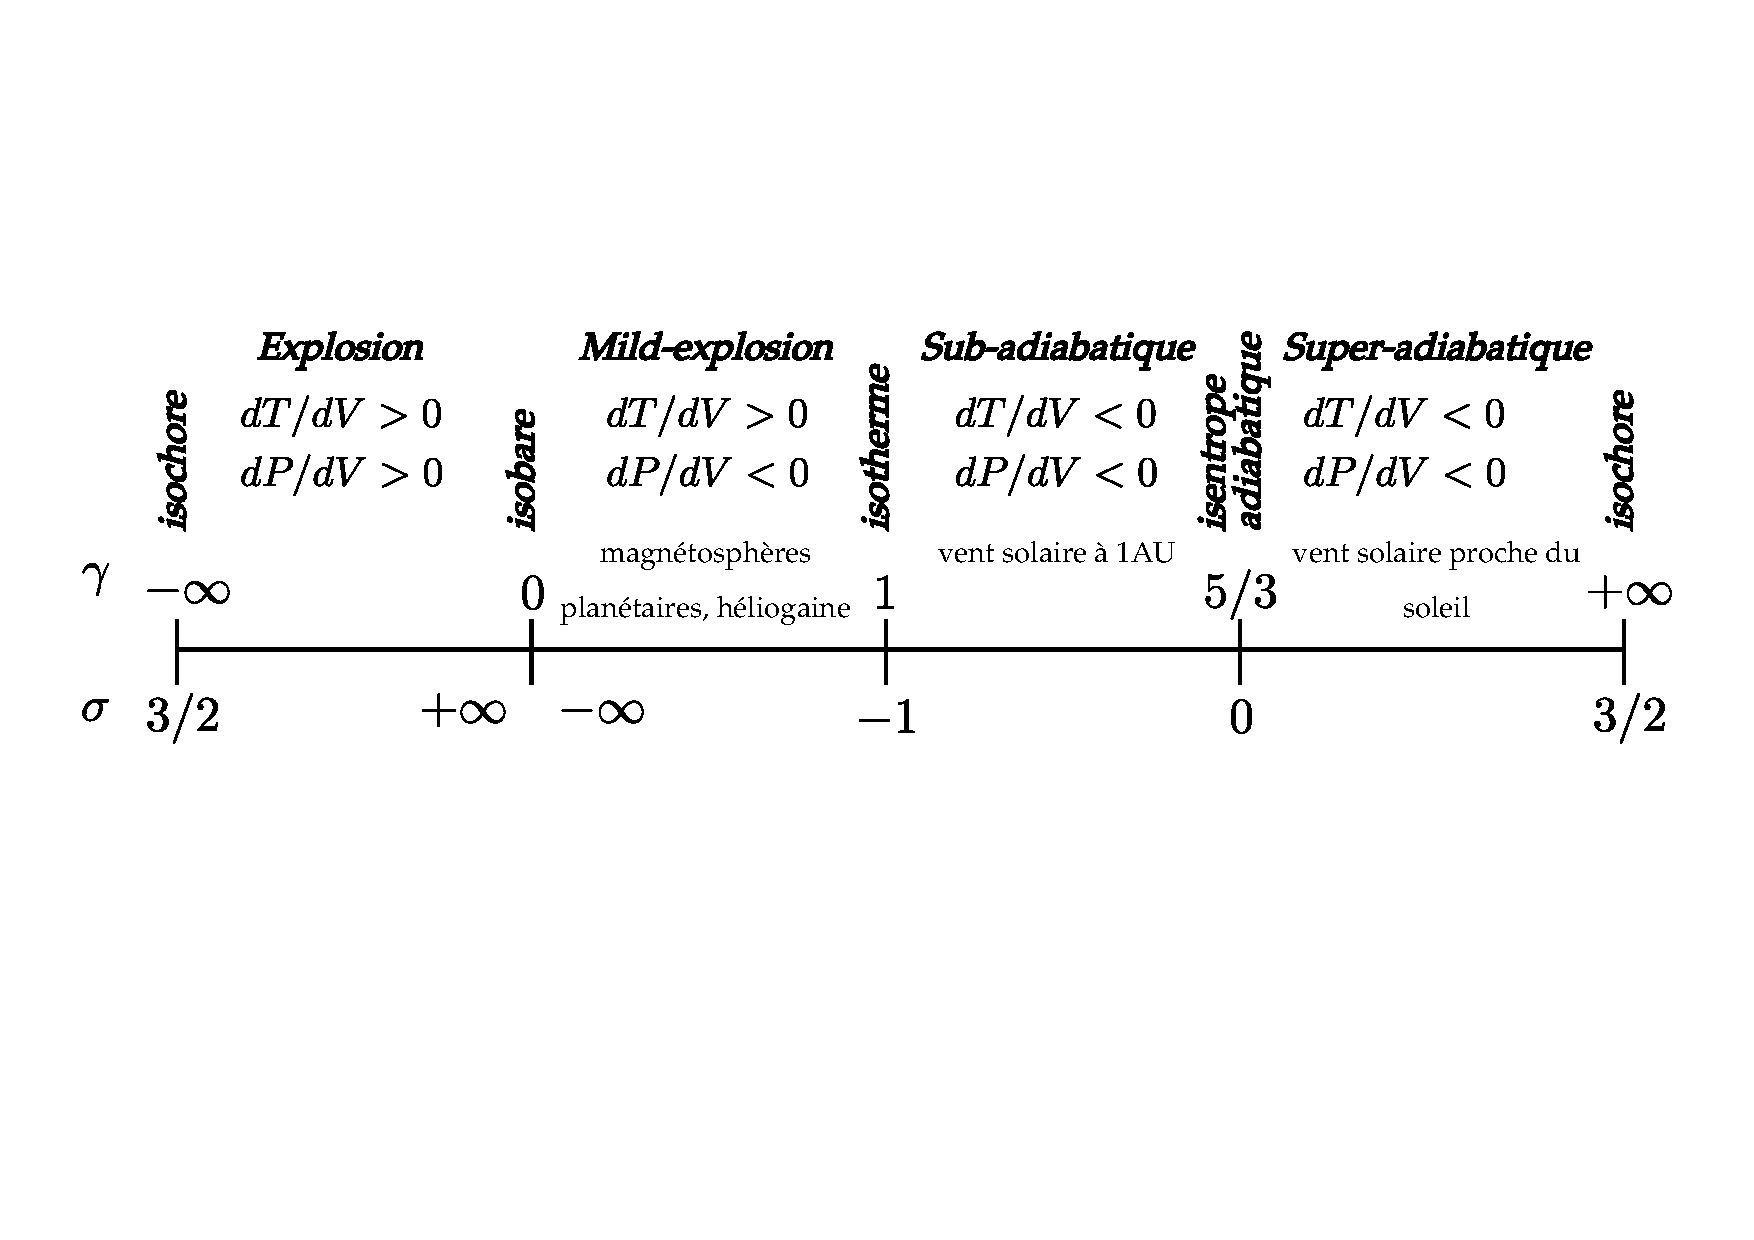
\includegraphics[width=0.9\linewidth,trim=1cm 8cm 1cm 5.5cm, clip=true]{./Part_1/images/schema_thermo.pdf}
\caption{Transformations thermodynamiques et intervalles en fonction du $\gamma$ du milieu [\cite{livadiotis_non-equilibrium_2012}] et du $\sigma$ [\cite{borel_thermodynamique_2005}], exemple de plasmas spatiaux [\cite{livadiotis_long-term_2018}]. Adiabatique et isentrope y sont confondus dans le cas réversible.}
\label{fig:schema_thermo}
\end{figure}

Dans le premier principe \eqref{eq:thermo_L1} et l'équation d'énergie interne \eqref{eq:thermo_u}, l'utilisation de $\sigma$ permet d'écrire : 
\begin{eqnarray}
\label{eq:thermo_sig_L1}    du &=& \dj \mathcal{Q} + \dj \mathcal{W} = \left(K+1\right) \dj \mathcal{W} = \left(\sigma \gamma + 1\right) \dj \mathcal{W} ,\\
\label{eq:thermo_sig_u}    d_t\left(\rho u\right) &=& -\left[\left(\sigma \gamma + 1\right) p + \rho u\right] \nabla \cdot \boldsymbol{v} ,\\
 \label{eq:thermo_sig_q}   &\Rightarrow& \nabla \cdot \boldsymbol{q} = -\rho T d_t s = \sigma \gamma p \nabla \cdot \boldsymbol{v}.
\end{eqnarray}
D'un autre côté, la relation entre $p$ et $V$ peut s'écrire $p \propto \rho^{\gamma}$. Cela donne l'équation : 
\begin{eqnarray}
 \label{eq:thermo_sig_p}   d_t p &=& -\gamma p \nabla \cdot \boldsymbol{v}.
\end{eqnarray}
Cette équation est compatible avec l'équation de pression du modèle fluide \eqref{eq:model_cpi_p} si :
\begin{eqnarray}
\label{eq:thermo_sig_gq}     \left(\frac{5}{3} -\gamma\right) p \nabla \cdot \boldsymbol{v} = -\frac{2}{3} \nabla \cdot \boldsymbol{q} 
\label{eq:thermo_sig_g}     &\Rightarrow& \left(\frac{5}{3} +\left(\frac{2}{3}\sigma-1\right)\gamma\right) p \nabla \cdot \boldsymbol{v} = 0 .
\end{eqnarray}
Par ces relations, on remarque que l'hypothèse polytrope peut nous permettre de fermer le modèle fluide au niveau du troisième moment $\boldsymbol{q}$ en injectant \eqref{eq:thermo_sig_q} dans l'équation de $p$ \eqref{eq:model_cpi_p}, ou au niveau du deuxième, $p$, en utilisant $\gamma$ et en injectant $p \propto \rho^{\gamma}$ dans \eqref{eq:model_cpi_v}\footnote{Usuellement, comme on cherche à fermer le modèle aussi tôt que possible, on ferme au niveau du deuxième moment. L'information sur le flux de chaleur est alors perdue d'où la confusion entre isentrope et polytrope.}. L'hypothèse adiabatique, isentrope si réversible, $\gamma=\gamma_a$ et $\nabla \cdot \boldsymbol{q}=0$, est retrouvée dans l'évolution fluide de $p$ si l'on se place dans le cadre d'un gaz parfait monoatomique $\gamma_a = 5/3$ d'après \eqref{eq:thermo_sig_gq}. Dans le cas isotherme, on retrouve dans \eqref{eq:thermo_sig_gq} ou \eqref{eq:thermo_sig_L1}, $\dj \mathcal{W} = - \dj \mathcal{Q}$, c'est-à-dire $du = 0$. En effet, la variation d'énergie interne d'un gaz parfait ne dépendant que de la température, ne peut qu'être nulle sous l'hypothèse d'isothermie. Les cas isochore (ou incompressible) et isobare sont plus délicats. Dans le cas isochore, le produit $\gamma \nabla \cdot \boldsymbol{v}$ qui apparaît dans toutes les expressions de \eqref{eq:thermo_sig_L1} à \eqref{eq:thermo_sig_g}, tend vers $\infty \times 0$. Dans le cas isobare, $\infty \times 0$ apparaît dès que $\sigma \gamma$ est présent dans l'équation. Ces limites du cas polytrope sont donc problématiques dans la définition de $u$. Elles doivent être traitées indépendamment. Dans le cas isochore, $\dj \mathcal{W} = 0$ et l'énergie interne ($d_t u + \nabla \cdot \boldsymbol{q} = 0 $) n'échange plus avec les énergies cinétique et magnétique. L'hypothèse isobare, quant à elle, ferme le système fluide au niveau de l'équation \eqref{eq:model_cpi_v}. L'équation d'énergie interne est alors  $\partial_t u + \nabla \cdot \left(u \boldsymbol{v} + \boldsymbol{q} + p_0 \boldsymbol{v}\right) = 0 $. Pour ces deux fermetures, l'énergie interne est conservée\footnote{La cascade d'énergie cinétique et magnétique peut alors être traitée indépendamment de celle d'énergie interne.  Cela a été fait dans le chapitre \ref{ch-11} dans le cadre incompressible.}.

Dans le cadre de la fermeture polytrope : $p = \frac{c_s^2}{\gamma} \rho$, avec $c^2_s = \frac{\partial p}{\partial \rho} \propto \rho^{\gamma-1}$ le carré de la vitesse thermique. Pour ce qui est de la variation d'énergie interne spécifique, elle devient :
\begin{eqnarray}
\label{eq:thermo_pol_du} d u &=& \left(\sigma \gamma+1\right) \frac{p}{\rho^2} d \rho =  \left(\sigma \gamma+1\right) \frac{p}{\rho^{\gamma}} \rho^{\gamma -2} d \rho \\
&=& \left\{ \begin{array}{lcl} \frac{\sigma \gamma+1}{\gamma-1} \frac{p}{\rho^{\gamma}} d\left( \rho^{\gamma-1} \right)  &\textrm{ si }&  \gamma \neq 1\\
\left(\sigma+1\right) \frac{p}{\rho} d \left(\ln{\rho}\right)  &\textrm{ si }&  \gamma = 1
\end{array} \right. .
\end{eqnarray}
Et par intégration :
\begin{eqnarray}
\label{eq:thermo_pol_u} u - u_I &=& \left\{ \begin{array}{lclcl} \frac{\sigma \gamma+1 }{\gamma-1} \frac{p}{\rho^{\gamma}} \left(\rho^{\gamma-1} - \rho_I^{\gamma-1}\right) &=& \frac{\sigma \gamma+1 }{\gamma-1} \frac{c_s^2}{\gamma} \left(1 - \left(\frac{\rho_I}{\rho}\right)^{\gamma-1}\right)  & \textrm{ si } & \gamma \neq 1\\
   \left(\sigma+1\right) \frac{p}{\rho} \ln \frac{\rho}{\rho_I} &=& \left(\sigma+1\right) c_s^2 \ln \frac{\rho}{\rho_I} &\textrm{ si }&  \gamma = 1 
   \end{array} \right. ,
\end{eqnarray} 
en notant $u_I$ et $\rho_I$ les constantes d'intégrations.
Dans le cas particulier de la fermeture isotherme : $\gamma = 1$, $\sigma = -1$, $p = c^2_s \rho$ avec $c_s$ constante et $du = 0$. 

\section{Thermodynamique et turbulence} \label{sec-112bis}

La cascade turbulente pourrait être, dans les plasmas spatiaux peu collisionnels, une réponse au problème du chauffage. En définissant le chauffage comme la variation de température et sachant que pour un gaz parfait, l'énergie interne ne dépend que de la température\footnote{Dans un gaz parfait, on suppose que les particules n'interagissent pas entre elles, donc qu'elles soient éloignées ou proches n'influera pas sur leur énergie individuelle. Par conséquent, l'énergie interne est indépendante de la densité. Cependant, la densité d'énergie interne dépendra de $\rho$ et $T$.}. Il est facile de définir le chauffage comme tout transfert d'énergie vers l'énergie interne, appelée aussi énergie thermique [\cite{cassak_pressure-strain_2022}]. Le terme de pression dans l'équation \eqref{eq:model_cpi_v} s'interprète alors comme les termes visqueux et résistifs abordés dans le Chapitre \ref{ch-11}, c'est-à-dire comme un terme "dissipatif". Mais, ce serait oublier que la cascade turbulente permet de faire le lien entre les grandes échelles, MHD où la validité de l'hypothèse de gaz parfait est cohérente puisque l'on néglige les interactions entre ions et électrons, et les petites échelles, cinétiques, où les interactions commencent à apparaître à travers le champ électromagnétique. Il manque donc un ingrédient à la définition du chauffage comme un transfert d'énergie vers l'énergie interne. Si l'on regarde la dissipation visqueuse ou résistive, elle vient réduire l'énergie du système, mais elle apparaît aussi dans l'équation d'entropie [\cite{eyink_cascades_2018}]. Chauffer ainsi va donc venir augmenter l'entropie du plasma. {\bf La définition du chauffage adaptée à l'étude de la turbulence est donc celle d'un transfert énergétique avec l'énergie interne impactant l'entropie. Le taux de cascade doit donc prendre en compte l'énergie étant transférée isentropiquement à l'énergie interne.}

Cette définition du chauffage justifie l'hypothèse proposée par [\cite{galtier_exact_2011}] que seul le terme de travail $\dj \mathcal{W}$ de l'énergie interne affecte la cascade dans la zone inertielle. Cette hypothèse revient à supposer une zone inertielle isentrope telle que $\sigma = 0$. Si le système global est fermé tel que $\gamma \neq \gamma_a$, le terme de chaleur $\dj \mathcal{Q}$ jouera un rôle aux autres échelles afin que les relations thermodynamiques soient respectées dans le système global. La fermeture considérée par [\cite{galtier_exact_2011}] est la fermeture isotherme qui dans l'hypothèse d'une zone inertielle isentrope implique :  $\gamma = 1$, $\sigma = 0$, $p = c^2_s \rho$ avec $c_s$ constante et $du = \dj \mathcal{W} \Rightarrow u-u_I = \frac{p}{\rho} \ln \frac{\rho}{\rho_I} $. On appellera cette fermeture, qui n'est valable que dans la zone inertielle, <<isentrope-isotherme>> afin d'expliciter la nuance existant entre l'isotherme basique tel que $du = 0$ et l'isotherme étudié dans le cadre d'une cascade isentrope. En suivant cette logique, je me suis intéressée dans [\cite{simon_general_2021}] à la fermeture <<isentrope-polytrope>> telle que $\sigma = 0$,  $p = \frac{c_s^2}{\gamma} \rho^{\gamma}$ et 
\begin{eqnarray}
\label{eq:thermo_ipol_u} u - u_I &=& \left\{ \begin{array}{lclcl} \frac{1 }{\gamma-1} \frac{p}{\rho^{\gamma}} \left(\rho^{\gamma-1} - \rho_I^{\gamma-1}\right) &=& \frac{+1 }{\gamma-1} \frac{c_s^2}{\gamma} \left(1 - \left(\frac{\rho_I}{\rho}\right)^{\gamma-1}\right)  & \textrm{ si } & \gamma \neq 1\\
    \frac{p}{\rho} \ln \frac{\rho}{\rho_I} &=&  c_s^2 \ln \frac{\rho}{\rho_I} &\textrm{ si }&  \gamma = 1 
   \end{array} \right. .
\end{eqnarray} 
Dans l'usage des formes explicites de l'énergie interne dans les calculs de lois exactes avec l'hypothèse polytrope, les constantes sont souvent annulées entre elles. Par exemple, dans le cas <<isentrope-polytrope>>, \cite{banerjee_kolmogorov-like_2014} considère comme forme explicite de l'énergie interne $ \rho u = \frac{1}{\left(\gamma-1\right)} p $. Contrairement à ce travail, nous avons choisi de maintenir une forme de compatibilité avec la fermeture <<isentrope-isotherme>> de \cite{galtier_exact_2011} (si $u = u_I$ alors $u = 0$) dans nos choix de constantes.

Sont résumés dans la \tabref{tab:fermetures}, les caractéristiques, dénominations et choix de constante des fermetures définies polytropiquement via $\sigma$ et $\gamma$ qui serviront par la suite. 
\begin{table}[!ht]
\begin{center}
\begin{tabular}{ c|c|c } 
Nom & Paramètres & Energie interne explicite\\
\hline
Polytrope (hors isotherme)  & $\{\sigma,\gamma \neq 1 \}$  & $ \frac{\sigma \gamma+1 }{\gamma-1} \frac{p}{\rho^{\gamma}} \left(\rho^{\gamma-1} - \rho_I^{\gamma-1}\right) $    \\
Isotherme  & $\{-1,1\}$ & $  u = 0$     \\
Isentrope-polytrope (hors isotherme) & $\{0,\gamma \neq 1\}$ & $ \frac{1 }{\gamma-1} \frac{p}{\rho^{\gamma}} \left(\rho^{\gamma-1} - \rho_I^{\gamma-1}\right)  $  \\
Isentrope-isotherme & $\{0,1\}$  & $ u = \frac{p}{\rho} \ln \frac{\rho}{\rho_I}$  \\
\end{tabular}
\end{center}
\caption{Fermetures et relations associées. La forme de l'énergie interne de l'isentrope-isotherme est calquée sur celle utilisée par \cite{galtier_exact_2011}. Les autres sont définies de telle sorte à maintenir une forme de compatibilité : si $u = u_I$ alors $u = 0$. Celle de l'isentrope-polytrope est donc légèrement différente de celle utilisée par \cite{banerjee_kolmogorov-like_2014}. $\frac{p}{\rho}$ peut aussi s'écrire $\frac{c_s^2}{\gamma}$ et $p \propto \rho^{\gamma}$. \label{tab:fermetures}}
\end{table}

\cite{aluie_conservative_2012} observent en détail la cascade d'énergie cinétique et magnétique dans différentes simulations subsoniques à transoniques. Le transfert cinétique-interne via la pression semble n'avoir lieu qu'à grande échelle dans une zone qu'ils appellent <<zone de conversion>>, à plus petites échelles cette contribution reste constante. Ils en déduisent un découplage des cascades d'énergie cinétique et d'énergie interne et l'existence d'une zone inertielle cinétique. \cite{eyink_cascades_2018} déduisent aussi, analytiquement, un effet à grande échelle de la pression qui permettrait d'alimenter des structures cohérentes et de réduire l'entropie à grande échelle. Cela induirait une cascade inverse d'entropie vers les grandes échelles et un équilibre s'établirait entre les cascades d'énergie totale et d'entropie. Aucun de ces résultats ne prouve que l'énergie interne ne cascade pas. Ne pas la prendre en compte dans l'estimation du taux de chauffage comme le propose \cite{hellinger_von_2018} est donc hasardeux et n'est justifiable que dans le cas subsonique où sa contribution semble mineure [\cite{andres_energy_2018,ferrand_compressible_2020}] ou à des échelles plus faibles que celle où l'impact de la pression semble majeur [\cite{aluie_conservative_2012}]. Etudier la cascade compressible dans une zone inertielle où la pression ne transférerait pas d'énergie vers l'énergie interne, c'est à dire $\nabla p = 0$ dans l'équation \eqref{eq:lin_cpi_v}, correspondrait à regarder une zone inertielle isobare. Au vu des observations, cela ne semble pas physiquement absurde, mais étant intéressés par l'impact de la pression sur la cascade turbulente totale, cette hypothèse réductrice n'a pas retenu notre intérêt. 


\section{Propriétés linéaires de la \ac{MHD} compressible}
\label{sec-123}

Dans le cadre de l'obtention d'une relation de dispersion compressible, on fermera le système avec la fermeture polytrope pour rester dans le cas le plus général possible. Ainsi, on utilise le système d'équations : 
\begin{eqnarray}
\label{eq:lin_cpi_r}\partial_t \rho + \nabla \cdot \left(\rho \boldsymbol{v}\right) &=& 0,\\
\label{eq:lin_cpi_v}\partial_t \left(\rho \boldsymbol{v}\right) + \nabla \cdot \left(\rho \boldsymbol{v}\boldsymbol{v} - \rho \boldsymbol{v_A}\boldsymbol{v_A}\right) +  \nabla p_*  &=& 0 \label{eq:model_1}, \\
\label{eq:lin_cpi_b}\partial_t \boldsymbol{v_A} -  \nabla \cdot \left(\boldsymbol{v_A}\boldsymbol{v} - \boldsymbol{v}\boldsymbol{v_A}\right) +  \boldsymbol{v}  \nabla \cdot \boldsymbol{v_A} -  \frac{\boldsymbol{v_A}}{2}  \nabla \cdot \boldsymbol{v} &=& 0 ,
\end{eqnarray}
fermé par $p\propto \rho^{\gamma}$. 
 
L'application de la méthode de linéarisation présentée dans le Chapitre \ref{ch-11} nous donne l'équation de dispersion suivante :
\begin{equation}
    \begin{pmatrix}
\label{eq:lin_cpi_eqdis}    \frac{\omega^2}{k^2_{\parallel} v^2_{A0}} - \left(1+\frac{\gamma}{2} \beta_0\right)  \frac{k^2_{\perp}}{k^2_{\parallel}} - 1 & 0 & - \frac{\gamma}{2} \beta_0  \frac{k_{\perp}}{k_{\parallel}} \\
    0 & \frac{\omega^2}{k^2_{\parallel} v^2_{A0}} - 1  & 0 \\
     - \frac{\gamma}{2} \beta_0  \frac{k_{\perp}}{k_{\parallel}}  & 0 &\frac{\omega^2}{k^2_{\parallel} v^2_{A0}} -  \frac{\gamma}{2} \beta_0   
    \end{pmatrix} 
    \cdot \begin{pmatrix}
    v^{1}_x \\ v^{1}_y \\ v^{1}_z
    \end{pmatrix} = 0
\end{equation}
avec $\beta_0 = \frac{2p_0}{\rho_0 v^2_{A0}}$ le paramètre $\beta$ linéarisé du plasma. 
La relation de dispersion est donnée par l'annulation du déterminant de la matrice, c'est-à-dire, :
\begin{eqnarray}
 \label{eq:lin_cpi_disp}   0 = \left(\frac{\omega^2}{k^2_{\parallel} v^2_{A0}} - 1 \right)\left(\frac{\omega^2}{k^2 v^2_{A0}} - \frac{1}{2} \left(1+ \frac{\gamma}{2} \beta_0 \pm \sqrt{\Delta}\right)\right)
\end{eqnarray}
avec $\Delta = \left(1- \frac{\gamma}{2} \beta_0\right)^2 +2 \gamma \beta_0\sin^2\theta  = \left(1+ \frac{\gamma}{2} \beta_0\right)^2 -2 \gamma \beta_0\cos^2\theta$ en notant $\theta$ l'angle entre $\boldsymbol{k}$ et $\boldsymbol{e_z}$. La première racine correspond au mode d'Alfvén incompressible et les deux autres aux modes magnétosonores rapide ($+$) et lent ($-$). Ces modes sont stables ($\omega$ est réel), puisque $\Delta > 0$ et $\frac{1}{2} \left(1+ \frac{\gamma}{2} \beta_0 \pm \sqrt{\Delta}\right)>0$. 

Ces modes et leur version cinétique influencent le développement de la cascade turbulente en interagissant les uns avec les autres [\cite{cho_compressible_2003,sharma_nonlinear_2011,andres_interplay_2017,brodiano_spatiotemporal_2021,galtier_fast_2023}]. Dans le vent solaire, quasi-incompressible, le mode d'Alfvén et la cascade associée sont dominants. Cependant, les simulations et des filtrages de spectres relevés dans la magnétogaine ou la couronne solaire montrent des spectres de types turbulents pour les ondes magnétosoniques. Les simulations sont des outils très utilisés pour essayer de comprendre la répartition des rôles des différents modes [\cite{brodiano_spatiotemporal_2021}] mais l'universalité des résultats est questionnable, les résultats étant dépendants du forçage (Alfvénique ou non) initiant la cascade.  

\newpage
\section{Synthèse sur le modèle compressible avec pression isotrope}
\label{synt-12}
\fcolorbox{blue}{white}{\begin{minipage}[c]{\linewidth}
\paragraph{Modèle : } 
\begin{eqnarray}
\label{eq:synth_cpi_r} \partial_t \rho + \nabla \cdot \left(\rho \boldsymbol{v}\right) &=& 0 ,\\
\label{eq:synth_cpi_v}  \partial_t \left(\rho \boldsymbol{v}\right) + \nabla \cdot \left(\rho \boldsymbol{v}\boldsymbol{v} - \rho \boldsymbol{v_A}\boldsymbol{v_A}\right) +  \nabla p_*  &=& 0  ,\\
\label{eq:synth_cpi_b} \partial_t \boldsymbol{v_A} -  \nabla \cdot \left(\boldsymbol{v_A}\boldsymbol{v} - \boldsymbol{v}\boldsymbol{v_A}\right) +  \boldsymbol{v}  \nabla \cdot \boldsymbol{v_A} -  \frac{\boldsymbol{v_A}}{2}  \nabla \cdot \boldsymbol{v} &=& 0 , \\
\label{eq:synth_cpi_cb} \boldsymbol{v_A}\cdot \nabla  \rho  + 2\rho \nabla \cdot \boldsymbol{v_A}  &=& 0.
\end{eqnarray}

\paragraph{Fermetures écrites dans le cadre général polytrope et formes explicites de l'énergie interne spécifique considérées (telles que $u_I =u\left(\rho = \rho_I\right) =  0$) : } 
\begin{equation}
    \frac{p}{\rho} = \frac{c_s^2}{\gamma}, \quad c_s^2 \propto \rho^{\gamma-1}, \quad \sigma = \frac{\nabla \cdot \boldsymbol{q}}{\gamma p\nabla \cdot \boldsymbol{v}} ,\nonumber
\end{equation}
\begin{itemize}
    \item cas polytrope hors isotherme : $u = \frac{\sigma \gamma+1 }{\gamma-1} \frac{p}{\rho^{\gamma}} \left(\rho^{\gamma-1} - \rho_I^{\gamma-1}\right)$,
    \item cas isotherme : $\sigma = -1$, $\gamma = 1$, $u = 0$ et $c_s$ constants,
    \item cas isentrope-polytrope hors isotherme : $\sigma = 0$ et  $u = \frac{ \gamma+1 }{\gamma-1} \frac{p}{\rho^{\gamma}} \left(\rho^{\gamma-1} - \rho_I^{\gamma-1}\right) $,
    \item cas isentrope-isotherme  : $\sigma = 0$, $\gamma = 1$, $c_s$ constant et $u = c_s^2 \ln{\frac{\rho}{\rho_I}}$.
\end{itemize}

\paragraph{Equation d'énergie interne :} 
\begin{eqnarray}
\label{eq:synth_cpi_u} &\text{Formulation générale : }& \partial_t \left(\rho u\right) +\nabla \cdot \left(\rho u \boldsymbol{v} + \boldsymbol{q}\right)   = - p \nabla \cdot \boldsymbol{v} ,\\
\label{eq:synth_L1_du} &\text{Premier principe thermo : }& du =  \dj \mathcal{Q} + \dj \mathcal{W} = Tds + \frac{p}{\rho^2} d\rho , \\
\label{eq:synth_L1_u} &\text{Formulation thermo : }& \partial_t \left(\rho u\right) +\nabla \cdot \left(\rho u \boldsymbol{v}\right) - \rho T d_t s  = - p \nabla \cdot \boldsymbol{v}, \\
\label{eq:synth_L1_compu} &\Rightarrow \text{ Compatibilité : }& \nabla \cdot \boldsymbol{q} =  - \rho T d_t s , \\
\label{eq:synth_pol_u} &\text{Formulation polytrope : }& \partial_t \left(\rho u\right) +\nabla \cdot \left(\rho u \boldsymbol{v}\right)   = - \left(\sigma \gamma + 1 \right)p \nabla \cdot \boldsymbol{v} .
\end{eqnarray}

\paragraph{Equation de pression : }
\begin{eqnarray}
\label{eq:synth_cpi_p} &\text{Modèle fluide non fermé : }& \partial_t p + \nabla \cdot \left(  p\boldsymbol{v} + \frac{2}{3}\boldsymbol{q}\right) + \frac{2}{3} p \nabla \cdot \boldsymbol{v}  = 0 ,\\
\label{eq:synth_pol_p} &\text{Fermeture polytrope ($p \propto \rho^{\gamma}$) : }& \partial_t p + \boldsymbol{v} \cdot \nabla p - \gamma p \nabla \cdot \boldsymbol{v} = 0 ,\\
\label{eq:synth_cpi_comp} &\Rightarrow \text{ Compatibilité : }& \left(\frac{5}{3} + \left(\frac{2}{3}\sigma -1\right) \gamma\right)\nabla \cdot \boldsymbol{v} = 0 .
\end{eqnarray}

\end{minipage}}

\fcolorbox{blue}{white}{\begin{minipage}[c]{\linewidth}
\paragraph{Relation de dispersion linéaire : }
\begin{eqnarray}
 0 = \left(\frac{\omega^2}{k^2_{\parallel} v^2_{A0}} - 1 \right)\left(\frac{\omega^2}{k^2 v^2_{A0}} - \frac{1}{2} \left(1+ \frac{\gamma}{2} \beta_0 \pm \sqrt{\left(1- \frac{\gamma}{2} \beta_0\right)^2 +2 \gamma \beta_0\sin^2\theta}\right)\right) .
\end{eqnarray}
La première racine correspond au mode d'Alfvén similaire à celui obtenu en incompressible et les deux autres aux modes magnétosonores rapide ($+$) et lent ($-$). 
\end{minipage}}


\chapitre{Décrire la cascade compressible}{ch-13}
\chapter{Décrire la cascade compressible}
\renewcommand\partie{\Partie\ Chapitre \thechapter}
\label{ch-13}

%\medskip
\minitoc  

\bigskip

La variation du résultat de l'estimation d'un indice polytropique dans différents types de plasmas spatiaux (voir \figref{fig:schema_thermo}, [\cite{livadiotis_thermodynamic_2018}]) vient motiver la dérivation d'une loi exacte polytrope pour étudier la cascade d'énergie totale dans ces milieux. L'objectif initial du travail présenté dans cette partie et dont la contribution originale analytique est introduite dans ce chapitre, était de dériver une loi exacte \ac{MHD} polytrope, une extension des modèles \ac{MHD} isothermes [\cite{banerjee_exact_2013,andres_alternative_2017,andres_exact_2018,ferrand_compact_2021}] et \ac{HD} polytrope [\cite{banerjee_kolmogorov-like_2014}] existants. La cascade y est décrite similairement à celle décrite par \cite{galtier_exact_2011} (cas \ac{HD} isotherme). Suite à la discussion sur les fermetures thermodynamiques résumée dans le Chapitre \ref{ch-12}, on peut dire que, dans ces articles, elle est supposée isentrope dans la zone inertielle. L'hypothèse d'une fermeture polytrope (resp. isotherme) avec une zone inertielle isentrope revient à la fermeture "isentrope-polytrope" (resp. isentrope-isotherme) discutée au Chapitre \ref{ch-12}.

La méthode de calcul envisagée pour atteindre l'objectif initial a en réalité permis d'obtenir une loi exacte générale valable pour toutes les fermetures du système tant que l'isentropie est imposée dans la zone inertielle. 
Ce travail dont l'application à la fermeture "isentrope-polytrope" répond à l'objectif initial est présenté dans la section \ref{sec-131}. 
Dans la section \ref{sec-132}, on détaillera l'impact des fermetures sur une autre formulation de la loi qui a émergée du travail de relaxation de l'hypothèse d'isotropie de pression qui sera présenté dans le Chapitre \ref{ch-21}. 
Bien après avoir atteint l'objectif initial, on s'est posé la question de l'impact du flux de chaleur (a priori attendu en dehors de la zone inertielle) et on l'a pris en compte dans la loi \acs{KHM} qui, ainsi, a réellement pris une dimension générale. Notre loi a alors adopté une troisième formulation qui sera présentée dans la section \ref{sec-133}. Des applications isobare, isotherme et polytrope y seront abordées en tant qu'exemples d'application clôturant ce travail de généralisation.

\section{Dérivation d'une loi exacte compressible générale pour décrire un écoulement turbulent polytrope}
\label{sec-131}

La méthode utilisée ici pour dériver une loi exacte compressible correspond à celle détaillée dans le cas incompressible et résumée dans la section \ref{synt-11}. La première étape est de définir une fonction de corrélation. La pluralité de possibilités est plus importante que dans le cas incompressible puisque cette fois la compression ($\rho \neq 0$) impacte les densités d'énergie : $E_{tot} = \frac{1}{2} \rho \boldsymbol{v}^2 + \frac{1}{2} \rho \boldsymbol{v_A}^2 + \rho u $. Pour l'énergie cinétique, la volonté de considérer une forme de type auto-corrélation, a inspiré des études \ac{HD} et \ac{MHD} considérant sa racine-carré en $\sqrt{\rho} \boldsymbol{v} $ [\cite{hellinger_spectral_2021}] tandis que d'autres ont privilégié le sens physique de la quantité de mouvement $\rho \boldsymbol{v}$ (ex : \cite{galtier_exact_2011}). Pour l'énergie magnétique, la question est la même : $\boldsymbol{B}$ [\cite{ferrand_compact_2021}] ou $\rho \boldsymbol{v_A}$ [\cite{andres_alternative_2017}] ? Et pour l'énergie interne, les choix présents dans la littérature ont été en partie orientés suivant le type de fermeture : dans le cas polytrope par exemple, la forme explicite de l'énergie interne spécifique peut s'écrire tel que le carré de la vitesse thermique, d'où $\rho \sqrt{u}$ [\cite{banerjee_kolmogorov-like_2014}] ou $\sqrt{\rho u}$ alors que, dans le cas isotherme [\cite{galtier_exact_2011}], le choix était plutôt orienté vers la conservation de son intégrité et de prendre $\rho$ en un point et $u$ en un autre. Trois possibilités ont été envisagées pour chaque type d'énergie (dont la forme est ici généralisée en $E_\mathcal{X} = \rho X^2$) : 
\begin{itemize}
    \item l'auto-corrélation : $\mathcal{R_{X}}_1 = \left<\sqrt{\rho'} X' \cdot \sqrt{\rho} X \right>$ de fonction incrémentale associée :  $\mathcal{S_{X}}_1 = \left<\left(\delta \left(\sqrt{\rho} X\right)\right)^2\right>$ puisque $\mathcal{S_{X}}_1 = 2\left<E_\mathcal{X}\right> - 2\mathcal{R_{X}}_1 $
    \item la moyenne de densité : $\mathcal{R_{X}}_2 = \frac{1}{2}\left< \left(\rho'+\rho\right) X' \cdot X \right>$ de fonction incrémentale associée :  $\mathcal{S_{X}}_2 = \left<\delta \left(\rho X\right) \cdot \delta X \right>$ 
    \item la corrélation avec la densité : $\mathcal{R_{X}}_3 = \frac{1}{2}\left< \rho' X^2 + \rho X'{}^2\right> $ de fonction incrémentale associée :  $\mathcal{S_{X}}_3 = \left<\delta \rho  \delta X^2 \right>$ 
\end{itemize}
Il s'avère qu'utiliser des formes prenant en compte des racines carrées a tendance à compliquer le calcul et le résultat. Les formes finalement choisies sont donc : $\mathcal{R}_{c} = \mathcal{R}_{c2} = \left<\frac{1}{4} \left(\rho'+\rho\right) \boldsymbol{v'} \cdot  \boldsymbol{v} \right>$, $\mathcal{R}_{m} = \mathcal{R}_{m2} = \left<\frac{1}{4} \left(\rho'+\rho\right) \boldsymbol{v'_A} \cdot  \boldsymbol{v_A} \right>$ et $\mathcal{R}_{u} = \mathcal{R}_{u3} = \frac{1}{2}\left< \rho' u + \rho u'\right> $. Ce choix concorde avec celui de \cite{andres_energy_2018} dont les résultats de simulation permettront l'étude dans les données in-situ du Chapitre \ref{ch-14} et serviront de base de comparaison afin de valider les résultats de simulations présentés dans la Partie \ref{part_3}.

Pour ce qui est du modèle considéré, la première idée était d'appliquer la méthode de calcul des lois exactes sur le modèle fermé par l'hypothèse $p \propto \rho^{\gamma}$, dans la lignée des dérivations compressibles effectuées par exemple par \cite{galtier_exact_2011} et \cite{andres_alternative_2017}. Mais il s'est avéré qu'un autre choix plus judicieux existait. En effet, comme pour obtenir l'équation d'énergie totale \eqref{eq:model_cpi_e}, nous pouvons obtenir une loi exacte <<générale>> en utilisant l'équation de densité d'énergie interne \eqref{eq:synth_cpi_u} et sans expliciter la forme de $p$ ni celle de $u$. En première approximation, l'hypothèse isentrope qui implique $\nabla \cdot \boldsymbol{q} = 0$ via l'équation de compatibilité \eqref{eq:synth_L1_compu}, a d'abord été posée. Ce travail fait partie des résultats publiés dans \cite{simon_general_2021}. La loi \acs{KHM} générale qui y est obtenue n'est alors valable que dans la zone inertielle où l'hypothèse isentrope est supposée effective et ne sert que d'étape de calcul vers une loi \acs{K41}. Dans une volonté de donner un résultat pour la loi \acs{KHM} générale valable pour toutes les échelles, nous prendrons en compte $\nabla \cdot \boldsymbol{q}$ dans cette section, mais nous garderons sa contribution brute, sans travail analytique en accord avec le cheminement chronologique voulu pour ce chapitre. 

Les équations considérées sont celles de densité de masse \eqref{eq:synth_cpi_r}, vitesse  \eqref{eq:synth_cpi_v}, induction \eqref{eq:synth_cpi_b} et énergie interne  \eqref{eq:synth_cpi_u} avec des termes de forçage et de dissipation définis comme dans le cas incompressible (voir \eqref{eq:synth_inc_v} et \eqref{eq:synth_inc_b}). Ainsi :
\begin{eqnarray}
\label{eq:turb_cpi_r} \partial_t \rho &=& - \nabla \cdot \left(\rho \boldsymbol{v}\right), \\
\label{eq:turb_cpi_v}\partial_t  \boldsymbol{v} &=&- \nabla \cdot \left(\boldsymbol{v}\boldsymbol{v}\right) + \boldsymbol{v} \nabla \cdot \boldsymbol{v}  + \frac{1}{\rho} \nabla \cdot \left(\rho \boldsymbol{v_A}\boldsymbol{v_A}\right) - \frac{1}{\rho}  \nabla p_*  + \boldsymbol{f_c} + \boldsymbol{d_c} ,\\
\label{eq:turb_cpi_b}\partial_t \boldsymbol{v_A} &=&   \nabla \cdot \left(\boldsymbol{v_A}\boldsymbol{v} - \boldsymbol{v}\boldsymbol{v_A}\right) -  \boldsymbol{v}  \nabla \cdot \boldsymbol{v_A} +  \frac{\boldsymbol{v_A}}{2}  \nabla \cdot \boldsymbol{v} + \boldsymbol{f_m} + \boldsymbol{d_m} ,\\
\label{eq:turb_cpi_u}\partial_t u &=& - \nabla \cdot \left(u \boldsymbol{v}\right) + u  \nabla \cdot \boldsymbol{v} -\frac{1}{\rho} \nabla \cdot \boldsymbol{q}  - \frac{p}{\rho}  \nabla \cdot \boldsymbol{v} .
\end{eqnarray}
\eqref{eq:turb_cpi_v} et \eqref{eq:turb_cpi_b} peuvent aussi s'écrire en prenant en compte \eqref{eq:turb_cpi_r} :
\begin{eqnarray}
\label{eq:turb_cpi_v2}\partial_t  \left(\rho\boldsymbol{v}\right) &=&- \nabla \cdot \left(\rho \boldsymbol{v}\boldsymbol{v}\right)  + \nabla \cdot \left(\rho \boldsymbol{v_A}\boldsymbol{v_A}\right) -  \nabla p_*  + \rho \boldsymbol{f_c} + \rho\boldsymbol{d_c} ,\\
\label{eq:turb_cpi_b2}\partial_t \left(\rho\boldsymbol{v_A}\right) &=&   \nabla \cdot \left(\rho \boldsymbol{v_A}\boldsymbol{v} - \rho \boldsymbol{v}\boldsymbol{v_A}\right) +  \rho \boldsymbol{v}  \nabla \cdot \boldsymbol{v_A} - \frac{1}{2} \rho\boldsymbol{v_A} \nabla \cdot \boldsymbol{v} + \rho\boldsymbol{f_m} + \rho\boldsymbol{d_m}.
\end{eqnarray}

Si l'on regarde la forme des fonctions de corrélation incrémentales associées aux formes des fonctions choisies, on peut s'attendre à pouvoir identifier les fonctions de structure $\left<\delta \left(\rho\boldsymbol{v}\right) \cdot \delta \boldsymbol{v} \delta \boldsymbol{v}\right>$, $\left<\delta \left(\rho\boldsymbol{v_A}\right) \cdot \delta \boldsymbol{v_A} \delta \boldsymbol{v}\right>$ et $\left<\delta \rho \delta u \delta \boldsymbol{v}\right>$ et, similairement au cas incompressible, $\left<\delta \left(\rho\boldsymbol{v_A}\right) \cdot \delta \boldsymbol{v} \delta \boldsymbol{v_A}\right>$ ou $\left<\delta \left(\rho\boldsymbol{v}\right) \cdot \delta \boldsymbol{v_A} \delta \boldsymbol{v_A}\right>$. Le calcul de l'évolution temporelle des fonctions de corrélation pour chaque canal énergétique nous donne en effet : 
\begin{itemize}
    \item Canal d'énergie cinétique : $\mathcal{R}_{c} = \frac{1}{4}\left<\left(\rho'+\rho\right)\boldsymbol{v'} \cdot \boldsymbol{v}\right>$
\begin{eqnarray}
\label{eq:turb_cpi_Rc} 4\partial_t \mathcal{R}_{c} &=& \left<\partial_t \left(\rho' \boldsymbol{v'} \right)\cdot  \boldsymbol{v}  + \rho' \boldsymbol{v'} \cdot  \partial_t \boldsymbol{v} + \partial_t \left(\rho \boldsymbol{v} \right)\cdot  \boldsymbol{v'}  + \rho \boldsymbol{v} \cdot  \partial_t \boldsymbol{v'} \right>\nonumber \\
&=&\nabla_{\boldsymbol{\ell}} \cdot \left<\delta \left(\rho\boldsymbol{v}\right) \cdot \delta \boldsymbol{v} \delta \boldsymbol{v} -\left(\delta \left(\rho\boldsymbol{v_A}\right) \cdot \delta \boldsymbol{v} \delta \boldsymbol{v_A} + \delta \left(\rho\boldsymbol{v}\right) \cdot \delta \boldsymbol{v_A} \delta \boldsymbol{v_A} \right)\right>\nonumber \\
&&+ \nabla_{\boldsymbol{\ell}} \cdot \left<\rho' \boldsymbol{v'_A}\cdot  \boldsymbol{v} \boldsymbol{v_A} -\rho \boldsymbol{v_A}\cdot  \boldsymbol{v'} \boldsymbol{v'_A}-\rho' \boldsymbol{v'} \cdot\boldsymbol{v_A}\boldsymbol{v'_A} +  \rho  \boldsymbol{v} \cdot\boldsymbol{v'_A}\boldsymbol{v_A}\right> \nonumber\\
&& +\left< \rho \boldsymbol{v} \cdot \delta \boldsymbol{v} \nabla' \cdot \boldsymbol{v'} -\rho' \boldsymbol{v'} \cdot \delta \boldsymbol{v} \nabla \cdot \boldsymbol{v} +2 \rho' \boldsymbol{v'} \cdot \delta \boldsymbol{v_A}\nabla \cdot \boldsymbol{v_A} - 2\rho \boldsymbol{v} \cdot \delta \boldsymbol{v_A}\nabla' \cdot \boldsymbol{v'_A}\right> \nonumber\\
&&+  \nabla_{\boldsymbol{\ell}} \cdot \left< \left(1+\frac{\rho'}{\rho}\right)p_*  \boldsymbol{v'} -  \left(1+\frac{\rho}{\rho'}\right)p'_*  \boldsymbol{v} \right>- \left<\frac{\rho'}{\rho} p_*  \boldsymbol{v'} \cdot \frac{\nabla \rho}{\rho} + \frac{\rho}{\rho'} p'_*  \boldsymbol{v} \cdot \frac{\nabla' \rho'}{\rho'} \right>\nonumber\\
&&+  \left<\left(\rho' + \rho\right)\left(\boldsymbol{v} \cdot \boldsymbol{f'_c} + \boldsymbol{v'} \cdot \boldsymbol{f_c}\right) \right>+ \left<\left(\rho' + \rho\right)\left(\boldsymbol{v} \cdot \boldsymbol{d'_c} + \boldsymbol{v'} \cdot \boldsymbol{d_c}\right)\right> .
\end{eqnarray}
    \item Canal d'énergie magnétique : $\mathcal{R}_{m} = \frac{1}{4}\left<\left(\rho'+\rho\right)\boldsymbol{v'_A} \cdot \boldsymbol{v_A}\right> $
\begin{eqnarray}
\label{eq:turb_cpi_Rm} 4\partial_t \mathcal{R}_{m} &=& \left<\partial_t \left(\rho' \boldsymbol{v'_A} \right)\cdot  \boldsymbol{v_A}  + \rho' \boldsymbol{v'_A} \cdot  \partial_t \boldsymbol{v_A} + \partial_t \left(\rho \boldsymbol{v_A} \right)\cdot  \boldsymbol{v'_A}  + \rho \boldsymbol{v_A} \cdot  \partial_t \boldsymbol{v'_A} \right> \nonumber\\
&=&\nabla_{\boldsymbol{\ell}} \cdot \left<\delta \left(\rho\boldsymbol{v_A}\right) \cdot \delta \boldsymbol{v_A} \delta \boldsymbol{v} \right> + \left<\left(\rho \boldsymbol{v_A} \cdot \delta \boldsymbol{v_A} -\frac{1}{2} \left(\rho'+\rho\right) \boldsymbol{v'_A} \cdot \boldsymbol{v_A}\right)\nabla' \cdot \boldsymbol{v'}\right>\nonumber\\
&&-  \left<\left(\rho' \boldsymbol{v'_A} \cdot \delta \boldsymbol{v_A} + \frac{1}{2} \left(\rho'+\rho\right) \boldsymbol{v'_A} \cdot \boldsymbol{v_A}\right)\nabla \cdot \boldsymbol{v}\right>\\
&& + \left<\left( \rho' \boldsymbol{v'_A} \cdot \boldsymbol{v} - \rho \boldsymbol{v} \cdot \boldsymbol{v'_A}  \right)\nabla \cdot \boldsymbol{v_A} \right> + \left<\left(\rho' \boldsymbol{v'} \cdot \boldsymbol{v_A} -  \rho \boldsymbol{v_A} \cdot \boldsymbol{v'} \right)\nabla' \cdot \boldsymbol{v'_A} \right>\nonumber\\
&&-\nabla_{\boldsymbol{\ell}} \cdot \left< \rho' \boldsymbol{v'_A}\cdot  \boldsymbol{v} \boldsymbol{v_A} - \rho \boldsymbol{v_A}\cdot  \boldsymbol{v'} \boldsymbol{v'_A}-\rho' \boldsymbol{v'} \cdot\boldsymbol{v_A}\boldsymbol{v'_A} +  \rho  \boldsymbol{v} \cdot\boldsymbol{v'_A}\boldsymbol{v_A}\right> \nonumber\\
&&+  \left<\left(\rho' + \rho\right)\left(\boldsymbol{v_A} \cdot \boldsymbol{f'_m} + \boldsymbol{v'_A} \cdot \boldsymbol{f_m}\right) \right>+ \left<\left(\rho' + \rho\right)\left(\boldsymbol{v_A} \cdot \boldsymbol{d'_m} + \boldsymbol{v'_A} \cdot \boldsymbol{d_m}\right)\right> . \nonumber
\end{eqnarray}
 \item Canal d'énergie interne :  $\mathcal{R}_{u} = \frac{1}{2}\left<\rho' u+\rho u'\right> $
\begin{eqnarray}
\label{eq:turb_cpi_Ru} 2\partial_t \mathcal{R}_{u} &=& \left<\partial_t \left(\rho'\right) u  + \rho' \partial_t u + \partial_t \left(\rho\right) u' + \rho \partial_t u'\right> \nonumber\\
&=&\nabla_{\boldsymbol{\ell}} \cdot \left<\delta \rho  \delta u \delta \boldsymbol{v} \right> + \left<  \rho \delta u \nabla \cdot \boldsymbol{v'}- \rho' \delta u \nabla \cdot \boldsymbol{v}\right> \nonumber\\
&&-\left< \rho' \frac{p}{\rho}   \nabla \cdot \boldsymbol{v}  + \rho \frac{p'}{\rho'}   \nabla' \cdot \boldsymbol{v'} \right> -\left<\frac{\rho}{\rho'}  \nabla' \cdot \boldsymbol{q'} + \frac{\rho'}{\rho}  \nabla \cdot \boldsymbol{q}  \right> .
\end{eqnarray}
\end{itemize}
D'où pour l'énergie totale avec $\mathcal{R} = \mathcal{R}_{c} + \mathcal{R}_{m} + \mathcal{R}_{u}$ :
\begin{equation}
\label{eq:turb_cpi_khm} \boxed{
\begin{array}{lcl}
{}_{[1]} \quad 4\partial_t \mathcal{R} &=& \nabla_{\boldsymbol{\ell}} \cdot \left<\left(\delta \left(\rho\boldsymbol{v}\right) \cdot \delta \boldsymbol{v}+ \delta \left(\rho\boldsymbol{v_A}\right) \cdot \delta \boldsymbol{v_A} \right)\delta \boldsymbol{v}  -\left(\delta \left(\rho\boldsymbol{v_A}\right) \cdot \delta \boldsymbol{v}  + \delta \left(\rho\boldsymbol{v}\right) \cdot \delta \boldsymbol{v_A}  \right) \delta \boldsymbol{v_A} \right>\\
{}_{[2]} && +\left< \left(\rho \boldsymbol{v} \cdot \delta \boldsymbol{v} +\rho \boldsymbol{v_A} \cdot \delta \boldsymbol{v_A} -\frac{1}{2} \left(\rho'+\rho\right) \boldsymbol{v'_A} \cdot \boldsymbol{v_A} \right) \nabla' \cdot \boldsymbol{v'} \right>\\
{}_{[3]} && -\left< \left(\rho' \boldsymbol{v'} \cdot \delta \boldsymbol{v} + \rho' \boldsymbol{v'_A} \cdot \delta \boldsymbol{v_A} + \frac{1}{2} \left(\rho'+\rho\right) \boldsymbol{v'_A} \cdot \boldsymbol{v_A}  \right)\nabla \cdot \boldsymbol{v}\right>\\
{}_{[4]} &&+ \left<\left(2 \rho' \boldsymbol{v'} \cdot \delta \boldsymbol{v_A}+\rho \boldsymbol{v} \cdot \boldsymbol{v'_A} - \rho' \boldsymbol{v'_A} \cdot \boldsymbol{v}  \right)\nabla \cdot \boldsymbol{v_A}\right> \\
{}_{[5]} &&- \left<\left(2\rho \boldsymbol{v} \cdot \delta \boldsymbol{v_A} -\rho' \boldsymbol{v'} \cdot \boldsymbol{v_A} +  \rho \boldsymbol{v_A} \cdot \boldsymbol{v'} \right)\nabla' \cdot \boldsymbol{v'_A}\right> \\
{}_{[6]} &&+ 2 \nabla_{\boldsymbol{\ell}} \cdot \left<\delta \rho  \delta u \delta \boldsymbol{v}\right> + 2\left<\left(\rho \delta u- \rho \frac{p'}{\rho'}\right)\nabla' \cdot \boldsymbol{v'}  - \left(\rho' \delta u + \rho' \frac{p}{\rho}\right) \nabla \cdot \boldsymbol{v} \right>\\
{}_{[7]} &&+  \nabla_{\boldsymbol{\ell}} \cdot \left< \left(1+\frac{\rho'}{\rho}\right)p_*  \boldsymbol{v'} -  \left(1+\frac{\rho}{\rho'}\right)p'_*  \boldsymbol{v} \right>- \left<\frac{\rho'}{\rho} p_*  \boldsymbol{v'} \cdot \frac{\nabla \rho}{\rho} + \frac{\rho}{\rho'} p'_*  \boldsymbol{v} \cdot \frac{\nabla' \rho'}{\rho'} \right>\\
{}_{[8]} &&-2\left<\frac{\rho}{\rho'}  \nabla' \cdot \boldsymbol{q'} + \frac{\rho'}{\rho}  \nabla \cdot \boldsymbol{q}  \right> \\
{}_{[9]}&&+  \left<\left(\rho' + \rho\right)\left(\boldsymbol{v} \cdot \boldsymbol{f'_c} + \boldsymbol{v'} \cdot \boldsymbol{f_c} + \boldsymbol{v_A} \cdot \boldsymbol{f'_m} + \boldsymbol{v'_A} \cdot \boldsymbol{f_m}\right) \right>\\
{}_{[10]}&&+ \left<\left(\rho' + \rho\right)\left(\boldsymbol{v} \cdot \boldsymbol{d'_c} + \boldsymbol{v'} \cdot \boldsymbol{d_c}+\boldsymbol{v_A} \cdot \boldsymbol{d'_m} + \boldsymbol{v'_A} \cdot \boldsymbol{d_m}\right)\right> .
\end{array}}
\end{equation} 
Cette loi \acs{KHM} est valable à toutes les échelles où est valable le modèle \ac{MHD}. Comme elle est obtenue à partir du modèle \ac{MHD} non fermé, elle est adaptable à toute fermeture et hypothèse thermodynamique considérées dans la zone inertielle. C'est le premier résultat majeur obtenu, il a été par la suite reformulé comme on le verra dans les sections suivantes. La ligne [1] contient la contribution à la cascade qui survit dans la limite incompressible, ces termes flux sont souvent nommés <<Yaglom compressible>>. Cette contribution est de type flux. Les lignes [2] à [8] contiennent les termes purement compressibles car ils s'annulent dans la limite incompressible. Les lignes [2] à [5] contiennent des termes dits <<sources>>, liés à l'effet de la dilation/compression du plasma sur les champs cinétiques et magnétiques (resp. $\nabla \cdot \boldsymbol{v}$ et $\nabla \cdot \boldsymbol{v_A}$). La ligne [6] contient des contributions d'énergie interne et de pression convectées par le champ de vitesse sous la forme d'un terme flux, qui semble indiquer l'existence d'une cascade d'énergie interne à travers les échelles, et de termes sources. La ligne [7] contient la contribution de pression totale qui peut être écrite en factorisant la pression magnétique en fonction du paramètre $\beta = p/p_m$ du plasma et qui contient la majorité des termes nommés <<hybrides>> par \cite{andres_alternative_2017} car il est possible de les écrire sous le format flux ou source. Cette ligne sera principalement affectée par les reformulations présentées dans les sections \ref{sec-132} et \ref{sec-133}. La ligne [8] contient la contribution du flux de chaleur qui sera abordée et reformulée dans la section \ref{sec-133}. Et, pour finir, les lignes [9] et [10] correspondent aux taux d'injection et de dissipation de l'énergie totale compressible. 

Dans le cadre d'une zone inertielle isentrope, il faut prendre en compte les lignes [1] à [7] dans le taux de cascade :
\begin{equation}
\boxed{
\begin{array}{lcl}
\label{eq:turb_elg_f1} -4\varepsilon &=& \nabla_{\boldsymbol{\ell}} \cdot \left<\left(\delta \left(\rho\boldsymbol{v}\right) \cdot \delta \boldsymbol{v}+ \delta \left(\rho\boldsymbol{v_A}\right) \cdot \delta \boldsymbol{v_A} \right)\delta \boldsymbol{v}  -\left(\delta \left(\rho\boldsymbol{v_A}\right) \cdot \delta \boldsymbol{v}  + \delta \left(\rho\boldsymbol{v}\right) \cdot \delta \boldsymbol{v_A}  \right) \delta \boldsymbol{v_A} \right>\\
&& +\left< \left(\rho \boldsymbol{v} \cdot \delta \boldsymbol{v} +\rho \boldsymbol{v_A} \cdot \delta \boldsymbol{v_A} -\frac{1}{2} \left(\rho'+\rho\right) \boldsymbol{v'_A} \cdot \boldsymbol{v_A} \right) \nabla' \cdot \boldsymbol{v'} \right>\\
&& -\left< \left(\rho' \boldsymbol{v'} \cdot \delta \boldsymbol{v} + \rho' \boldsymbol{v'_A} \cdot \delta \boldsymbol{v_A} + \frac{1}{2} \left(\rho'+\rho\right) \boldsymbol{v'_A} \cdot \boldsymbol{v_A}  \right)\nabla \cdot \boldsymbol{v}\right>\\
&&+ \left<\left(2 \rho' \boldsymbol{v'} \cdot \delta \boldsymbol{v_A}+\rho \boldsymbol{v} \cdot \boldsymbol{v'_A} - \rho' \boldsymbol{v'_A} \cdot \boldsymbol{v}  \right)\nabla \cdot \boldsymbol{v_A}\right>\\
&&- \left<\left(2\rho \boldsymbol{v} \cdot \delta \boldsymbol{v_A} -\rho' \boldsymbol{v'} \cdot \boldsymbol{v_A} +  \rho \boldsymbol{v_A} \cdot \boldsymbol{v'} \right)\nabla' \cdot \boldsymbol{v'_A}\right> \\
&&+ 2 \nabla_{\boldsymbol{\ell}} \cdot \left<\delta \rho  \delta u \delta \boldsymbol{v}\right> + 2\left<\left(\rho \delta u- \rho \frac{p'}{\rho'}\right)\nabla' \cdot \boldsymbol{v'}  - \left(\rho' \delta u + \rho' \frac{p}{\rho}\right) \nabla \cdot \boldsymbol{v} \right>\\
&&+  \nabla_{\boldsymbol{\ell}} \cdot \left< \left(1+\frac{\rho'}{\rho}\right)p_*  \boldsymbol{v'} -  \left(1+\frac{\rho}{\rho'}\right)p'_*  \boldsymbol{v} \right>- \left<\frac{\rho'}{\rho} p_*  \boldsymbol{v'} \cdot \frac{\nabla \rho}{\rho} + \frac{\rho}{\rho'} p'_*  \boldsymbol{v} \cdot \frac{\nabla' \rho'}{\rho'} \right>.
\end{array}}
\end{equation} 
On obtient ainsi la <<loi exacte générale de type \acs{K41} dans le cadre d'une zone inertielle supposée isentrope>>. Grâce au premier principe de la thermodynamique \eqref{eq:synth_L1_du} qui peut alors s'écrire $\rho^2 \partial u = p \partial \rho $, on peut reformuler le dernier terme en fonction de l'énergie interne et du paramètre caractéristique en physique des plasmas $\beta = p/p_m$ local :
\begin{eqnarray}
\label{eq:turb_ref_beta}    \left<\frac{\rho'}{\rho} p_*  \boldsymbol{v'} \cdot \frac{\nabla \rho}{\rho} \right.&+& \left.\frac{\rho}{\rho'} p'_*  \boldsymbol{v} \cdot \frac{\nabla' \rho'}{\rho'} \right> = \left<\left(1+\frac{p_m}{p}\right)\rho' \boldsymbol{v'} \cdot \nabla u + \left(1+\frac{p'_m}{p'}\right)\rho \boldsymbol{v} \cdot \nabla' u'\right>\nonumber \\ &=& \nabla_{\boldsymbol{\ell}} \cdot \left<\rho u' \boldsymbol{v} - \rho' u \boldsymbol{v'}\right> + \left<\frac{1}{\beta}\nabla\cdot\left(\rho'  u \boldsymbol{v'}\right)  + \frac{1}{\beta'}\nabla'\cdot\left(\rho u'\boldsymbol{v}\right)   \right> .
\end{eqnarray}
On retrouve ainsi le résultat général publié et analysé dans \cite{simon_general_2021} (équation 18).

 L'injection de la fermeture isentrope-polytrope dans la loi \eqref{eq:turb_elg_f1} permet de répondre à l'objectif initial : trouver une loi exacte \ac{MHD} polytrope. Le résultat s'obtient directement et s'écrit, dans le cas $\gamma \neq 1$ (car on y injecte l'expression explicite de l'énergie interne) en fonction de $\gamma$ et $c^2_s$, : 
\begin{equation}
\label{eq:turb_elpol_f1}
\boxed{
\begin{array}{rcl}
-4\varepsilon &=& \nabla_{\boldsymbol{\ell}} \cdot \left<\left(\delta \left(\rho\boldsymbol{v}\right) \cdot \delta \boldsymbol{v}+ \delta \left(\rho\boldsymbol{v_A}\right) \cdot \delta \boldsymbol{v_A} \right)\delta \boldsymbol{v}  -\left(\delta \left(\rho\boldsymbol{v_A}\right) \cdot \delta \boldsymbol{v}  + \delta \left(\rho\boldsymbol{v}\right) \cdot \delta \boldsymbol{v_A}  \right) \delta \boldsymbol{v_A} \right>\\
&& +\left< \left(\rho \boldsymbol{v} \cdot \delta \boldsymbol{v} +\rho \boldsymbol{v_A} \cdot \delta \boldsymbol{v_A} -\frac{1}{2} \left(\rho'+\rho\right) \boldsymbol{v'_A} \cdot \boldsymbol{v_A} \right) \nabla' \cdot \boldsymbol{v'} \right>\\
&& -\left< \left(\rho' \boldsymbol{v'} \cdot \delta \boldsymbol{v} + \rho' \boldsymbol{v'_A} \cdot \delta \boldsymbol{v_A} + \frac{1}{2} \left(\rho'+\rho\right) \boldsymbol{v'_A} \cdot \boldsymbol{v_A}  \right)\nabla \cdot \boldsymbol{v}\right>\\
&&+ \left<\left(2 \rho' \boldsymbol{v'} \cdot \delta \boldsymbol{v_A}+\rho \boldsymbol{v} \cdot \boldsymbol{v'_A} - \rho' \boldsymbol{v'_A} \cdot \boldsymbol{v}  \right)\nabla \cdot \boldsymbol{v_A}\right>\\
&&- \left<\left(2\rho \boldsymbol{v} \cdot \delta \boldsymbol{v_A} -\rho' \boldsymbol{v'} \cdot \boldsymbol{v_A} +  \rho \boldsymbol{v_A} \cdot \boldsymbol{v'} \right)\nabla' \cdot \boldsymbol{v'_A}\right> \\
&&+ \frac{2}{\gamma\left(\gamma-1\right)} \nabla_{\boldsymbol{\ell}} \cdot \left<\delta \rho  \delta c^2_s \delta \boldsymbol{v}\right> + \frac{2}{\gamma} \left<\rho \left(\frac{1}{\gamma-1} \delta c^2_s - c'{}^2_s\right)\nabla' \cdot \boldsymbol{v'}  - \rho' \left(\frac{1}{\gamma-1}\delta c^2_s + c^2_s\right) \nabla \cdot \boldsymbol{v} \right>\\
&&+  \nabla_{\boldsymbol{\ell}} \cdot \left< \left(\rho+\rho'\right) \left(\frac{c^2_s}{\gamma}+\frac{\boldsymbol{v_A}^2}{2}\right) \boldsymbol{v'} -  \left(\rho+\rho'\right) \left(\frac{c'{}^2_s}{\gamma}+\frac{\boldsymbol{v'_A}^2}{2}\right)  \boldsymbol{v} \right>\\
&&- \left<\rho' \left(\frac{c^2_s}{\gamma}+\frac{\boldsymbol{v_A}^2}{2}\right)  \boldsymbol{v'} \cdot \frac{\nabla \rho}{\rho} + \rho \left(\frac{c'{}^2_s}{\gamma}+\frac{\boldsymbol{v'_A}^2}{2}\right)  \boldsymbol{v} \cdot \frac{\nabla' \rho'}{\rho'} \right>.
\end{array}}
\end{equation} 
On remarque que la partie constante de l'énergie interne dépendant de $\rho_I$ ne survit pas étant donné que cette énergie n'apparaît que sous forme incrémentale. C'est aussi le cas avec la reformulation \eqref{eq:turb_ref_beta} où l'énergie interne apparaît dérivée. En considérant $\boldsymbol{v_A} = 0$, on peut trouver une loi exacte pour le modèle \ac{HD} compressible polytrope :  
\begin{eqnarray}
-4\varepsilon &=& \nabla_{\boldsymbol{\ell}} \cdot \left<\left(\delta \rho\boldsymbol{v}\right) \cdot \delta \boldsymbol{v}\delta \boldsymbol{v} + \frac{2}{\gamma\left(\gamma-1\right)} \delta \rho  \delta c^2_s \delta \boldsymbol{v}\right> +\left< \rho \boldsymbol{v} \cdot \delta \boldsymbol{v}  \nabla' \cdot \boldsymbol{v'} - \rho' \boldsymbol{v'} \cdot \delta \boldsymbol{v} \nabla \cdot \boldsymbol{v}\right>\nonumber\\
&&+   \frac{2}{\gamma} \left<\rho \left(\frac{1}{\gamma-1} \delta c^2_s - c'{}^2_s\right)\nabla' \cdot \boldsymbol{v'}  - \rho' \left(\frac{1}{\gamma-1}\delta c^2_s + c^2_s\right) \nabla \cdot \boldsymbol{v} \right>\\
&&+  \nabla_{\boldsymbol{\ell}} \cdot \left< \left(\rho+\rho'\right) \frac{c^2_s}{\gamma} \boldsymbol{v'} -  \left(\rho+\rho'\right) \frac{c'{}^2_s}{\gamma}  \boldsymbol{v} \right> - \left<\rho' \frac{c^2_s}{\gamma}  \boldsymbol{v'} \cdot \frac{\nabla \rho}{\rho} + \rho \frac{c'{}^2_s}{\gamma} \boldsymbol{v} \cdot \frac{\nabla' \rho'}{\rho'} \right> .\nonumber
\end{eqnarray} 
On n'y reconnaît pas la loi proposée par \cite{banerjee_kolmogorov-like_2014} car ces derniers considèrent comme fonction de corrélation pour l'énergie interne : $\left<\frac{\rho c_s c'_s}{\gamma\left(\gamma-1\right)}\right>$. Passer de $\left<\frac{\rho c'{}^2_s }{\gamma\left(\gamma-1\right)}\right>$ à $\left<\frac{\rho c_s c'_s}{\gamma\left(\gamma-1\right)}\right>$ n'a pas été obtenu. Dans les essais effectués, on finissait toujours par supprimer la contribution de l'une et la remplacer par celle de l'autre. L'étude de la convergence de ces différentes formes de fonction de corrélation dans des simulations n'a pas été traitée dans ce travail.

Dans le cas de la fermeture isentrope-isotherme, on peut aussi obtenir un résultat rapidement à partir de \eqref{eq:turb_elg_f1} et après quelques manipulations et introduction d'autres notations, il est possible de retrouver la loi proposée par \cite{andres_alternative_2017} comme le montre \cite{simon_general_2021}.

\section{Reformulation de la loi \acs{K41} générale dépendant d'une pression isotrope}
\label{sec-132}

Dans le Chapitre \ref{ch-21}, nous dériverons une loi exacte de type \acs{K41} pour un modèle où l'isotropie de pression sera relaxée. Y imposer, après obtention, l'isotropie de pression, nous apporte la formulation suivante pour la loi générale \eqref{eq:turb_elg_f1} : 
\begin{equation}
\boxed{
\begin{array}{lcl}
\label{eq:turb_elg_f2}-4\varepsilon &=& \nabla_{\boldsymbol{\ell}} \cdot \left<\left(\delta \left(\rho\boldsymbol{v}\right) \cdot \delta \boldsymbol{v}+ \delta \left(\rho\boldsymbol{v_A}\right) \cdot \delta \boldsymbol{v_A}\right) \delta \boldsymbol{v}  -\left(\delta \left(\rho\boldsymbol{v_A}\right) \cdot \delta \boldsymbol{v}  + \delta \left(\rho\boldsymbol{v}\right) \cdot \delta \boldsymbol{v_A}  \right) \delta \boldsymbol{v_A} \right>\\
&& + \nabla_{\boldsymbol{\ell}} \cdot \left<\delta \rho  \left(2\delta u - \delta \left(\frac{p_*}{\rho}\right)\right)\delta \boldsymbol{v}\right> \\
&& +\left< \left(\rho \boldsymbol{v} \cdot \delta \boldsymbol{v} +\frac{1}{2} \rho \boldsymbol{v_A} \cdot \delta \boldsymbol{v_A} -\frac{1}{2} \boldsymbol{v_A} \cdot \delta \left(\rho \boldsymbol{v_A}\right) + 2\rho \left(\delta u - \delta \left(\frac{p}{\rho}\right)\right) \right) \nabla' \cdot \boldsymbol{v'} \right>\\
&& -\left<\left( \rho' \boldsymbol{v'} \cdot \delta \boldsymbol{v} +\frac{1}{2} \rho' \boldsymbol{v'_A} \cdot \delta \boldsymbol{v_A} -\frac{1}{2} \boldsymbol{v'_A} \cdot \delta \left(\rho \boldsymbol{v_A}\right) + 2\rho' \left(\delta u - \delta \left(\frac{p}{\rho}\right)\right)  \right)\nabla \cdot \boldsymbol{v}\right>\\
&&+ \left<\left(2 \rho' \boldsymbol{v'} \cdot \delta \boldsymbol{v_A}+ \delta\left(\rho \boldsymbol{v}\right) \cdot \boldsymbol{v'_A} - \rho' \boldsymbol{v'_A} \cdot \delta \boldsymbol{v}  \right)\nabla \cdot \boldsymbol{v_A}\right>\\
&&- \left<\left(2\rho \boldsymbol{v} \cdot \delta \boldsymbol{v_A} + \delta\left(\rho \boldsymbol{v}\right) \cdot \boldsymbol{v_A} - \rho \boldsymbol{v_A} \cdot \delta \boldsymbol{v}  \right)\nabla' \cdot \boldsymbol{v'_A}\right> \\
&&+  \left< \left(\frac{p_*}{\rho} \delta \rho - \rho \delta \left(\frac{p_*}{\rho}\right)  \right)\boldsymbol{v} \cdot \frac{\nabla' \rho'}{\rho'} - \left(\frac{p'_*}{\rho'} \delta \rho - \rho' \delta \left(\frac{p_*}{\rho}\right)  \right)  \boldsymbol{v'} \cdot \frac{\nabla \rho}{\rho} \right>.
\end{array}}
\end{equation} 
Cette formulation  est plus élégante que la précédente, car les termes flux apparaissent tous sous la forme de fonctions de structure grâce à l'introduction de $\left<\delta \rho \delta \left(\frac{p_*}{\rho}\right) \delta \boldsymbol{v}\right>$ et les termes sources s'écrivent tous sous une forme généralisée du type $\left<X \delta Y \nabla' Z'\right>$ ou  $\left<X' \delta Y \nabla Z\right>$ avec l'opération entre $\nabla$ et $Z$ pouvant être une divergence si $Z$ est une quantité vectorielle (ex : $\boldsymbol{v}$) ou un gradient ($\frac{\nabla \rho}{\rho} = \nabla \left(\ln \rho\right)$). Cette forme rend évident qu'en $\boldsymbol{\ell} = 0$, $\varepsilon = 0$. Le passage d'une forme à l'autre s'effectue en remarquant que les contributions de pression (notée $\varepsilon_{p}$) et de pression magnétique (notée $\varepsilon_{pm}$) peuvent s'écrire : 
\begin{eqnarray}
\label{eq:turb_ref_p} -4\varepsilon_{p} &=&\nabla_{\boldsymbol{\ell}} \cdot \left<\left(1+\frac{\rho'}{\rho}\right) p \boldsymbol{v'} - \left(1+\frac{\rho}{\rho'}\right)p'\boldsymbol{v} \right>  -2\left<\rho  \frac{p'}{\rho'} \nabla \cdot \boldsymbol{v'} + \rho' \frac{p}{\rho} \nabla \cdot \boldsymbol{v}\right> \nonumber\\
&=& - \nabla_{\boldsymbol{\ell}} \cdot \left<\delta \rho  \delta \frac{p}{\rho} \delta \boldsymbol{v} \right>  +   \left<2  \rho' \delta \left(\frac{p}{\rho}\right) \nabla \cdot \boldsymbol{v} - 2  \rho \delta \left(\frac{p}{\rho}\right) \nabla' \cdot \boldsymbol{v'}-\rho \frac{p'}{\rho'} \boldsymbol{v} \cdot \frac{\nabla'\rho'}{\rho'} - \rho' \frac{p}{\rho} \boldsymbol{v'} \cdot \frac{\nabla\rho}{\rho} \right>\nonumber\\ 
&&+ \left<\left(\delta \rho \frac{p_*}{\rho} - \rho \delta \left(\frac{p}{\rho}\right)\right)\boldsymbol{v} \cdot \frac{\nabla' \rho'}{\rho'} - \left(\delta \rho \frac{p'}{\rho'} - \rho' \delta \left(\frac{p_*}{\rho}\right)\right)\boldsymbol{v'} \cdot \frac{\nabla \rho}{\rho}\right>, \\
% \end{eqnarray}
% \begin{eqnarray}
\label{eq:turb_ref_pm}-4\varepsilon_{pm} &=&  \nabla_{\boldsymbol{\ell}} \cdot \left<\left(1+\frac{\rho'}{\rho}\right) p_m \boldsymbol{v'} - \left(1+\frac{\rho}{\rho'}\right)p'_m\boldsymbol{v} \right> - \left<\rho \frac{p'_m}{\rho'} \boldsymbol{v} \cdot \frac{\nabla'\rho'}{\rho'} + \rho' \frac{p_m}{\rho} \boldsymbol{v'} \cdot \frac{\nabla\rho}{\rho}\right> \nonumber\\
    &&+\left<\left(\rho \boldsymbol{v_A} \cdot \delta \boldsymbol{v_A} - \frac{1}{2}\left(\rho' + \rho\right) \boldsymbol{v'_A} \cdot \boldsymbol{v_A}\right)\nabla' \cdot \boldsymbol{v'} - \left(\rho' \boldsymbol{v'_A} \cdot \delta \boldsymbol{v_A} + \frac{1}{2}\left(\rho' + \rho\right) \boldsymbol{v'_A} \cdot \boldsymbol{v_A}\right)\nabla \cdot \boldsymbol{v}\right>\nonumber\\
    &=&- \nabla_{\boldsymbol{\ell}} \cdot \left<\delta \rho  \delta \frac{p_m}{\rho} \delta \boldsymbol{v} \right> + \left<\left(\delta \rho \frac{p_m}{\rho} - \rho \delta \left(\frac{p_m}{\rho}\right)\right)\boldsymbol{v} \cdot \frac{\nabla' \rho'}{\rho'} - \left(\delta \rho \frac{p'_m}{\rho'} - \rho' \delta \left(\frac{p_m}{\rho}\right)\right)\boldsymbol{v'} \cdot \frac{\nabla \rho}{\rho}\right>\nonumber\\
    &&+\frac{1}{2}\left<\left(\rho \boldsymbol{v_A} \cdot \delta \boldsymbol{v_A} - \boldsymbol{v_A} \cdot \delta \left(\rho \boldsymbol{v_A}\right)\right)\nabla' \cdot \boldsymbol{v'} - \left(\rho' \boldsymbol{v'_A} \cdot \delta \boldsymbol{v_A} - \boldsymbol{v'_A} \cdot \delta \left(\rho \boldsymbol{v_A}\right)\right)\nabla \cdot \boldsymbol{v}\right>.
\end{eqnarray}

Dans le cas isentrope-polytrope avec $\gamma \neq 1$, $\delta \left(u - p/\rho\right) = \delta [\left(2-\gamma\right)\frac{c^2_s}{\gamma\left(\gamma-1\right)}] = \left(2-\gamma\right)\delta u$ et de même, $\delta \left(2u - p/\rho\right) = \left(3-\gamma\right)\delta u$. Dans le cas isentrope-isotherme, c'est-à-dire avec $\gamma = 1$ et $c_s$ constant, $\delta \left(u - p/\rho\right) = \delta u = \left(2-\gamma\right)\delta u$ et  $\delta \left(2u - p/\rho\right) = \left(3-\gamma\right)\delta u$. De plus, $p_*/\rho = \left(1+\beta\right) \boldsymbol{v_A}^2/2 $. Ainsi, on peut déduire de \eqref{eq:turb_elg_f2}, une formulation de la loi exacte isentrope-polytrope valable pour tout $\gamma$, incluant donc la fermeture isentrope-isotherme, et dépendant de $u$, $\gamma$ et $\beta$ : 
\begin{equation}
\boxed{
\begin{array}{lcl}
\label{eq:turb_elpol_f2}-4\varepsilon &=& \nabla_{\boldsymbol{\ell}} \cdot \left<\left(\delta \left(\rho\boldsymbol{v}\right) \cdot \delta \boldsymbol{v}+ \delta \left(\rho\boldsymbol{v_A}\right) \cdot \delta \boldsymbol{v_A}\right) \delta \boldsymbol{v}  -\left(\delta \left(\rho\boldsymbol{v_A}\right) \cdot \delta \boldsymbol{v}  + \delta \left(\rho\boldsymbol{v}\right) \cdot \delta \boldsymbol{v_A}  \right) \delta \boldsymbol{v_A} \right>\\
&& + \nabla_{\boldsymbol{\ell}} \cdot \left<\delta \rho  \delta \left(\left(3-\gamma\right)u - \frac{\boldsymbol{v_A}^2}{2}\right)\delta \boldsymbol{v}\right> \\
&& +\left< \left(\rho \boldsymbol{v} \cdot \delta \boldsymbol{v} +\frac{1}{2} \rho \boldsymbol{v_A} \cdot \delta \boldsymbol{v_A} -\frac{1}{2} \boldsymbol{v_A} \cdot \delta \left(\rho \boldsymbol{v_A}\right) + 2 \left(2-\gamma\right)\rho \delta u \right) \nabla' \cdot \boldsymbol{v'} \right>\\
&& -\left< \left(\rho' \boldsymbol{v'} \cdot \delta \boldsymbol{v} +\frac{1}{2} \rho' \boldsymbol{v'_A} \cdot \delta \boldsymbol{v_A} -\frac{1}{2} \boldsymbol{v'_A} \cdot \delta \left(\rho \boldsymbol{v_A}\right) + 2\left(2-\gamma\right)\rho' \delta u   \right)\nabla \cdot \boldsymbol{v}\right>\\
&&+ \left<\left(2 \rho' \boldsymbol{v'} \cdot \delta \boldsymbol{v_A}+ \delta\left(\rho \boldsymbol{v}\right) \cdot \boldsymbol{v'_A} - \rho' \boldsymbol{v'_A} \cdot \delta \boldsymbol{v}  \right)\nabla \cdot \boldsymbol{v_A}\right>\\
&&- \left<\left(2\rho \boldsymbol{v} \cdot \delta \boldsymbol{v_A} + \delta\left(\rho \boldsymbol{v}\right) \cdot \boldsymbol{v_A} - \rho \boldsymbol{v_A} \cdot \delta \boldsymbol{v}  \right)\nabla' \cdot \boldsymbol{v'_A}\right> \\
&&+  \left< \left(\frac{\boldsymbol{v_A}^2}{2} \left(1+\beta\right) \delta \rho - \rho \delta \left(\frac{\boldsymbol{v_A}^2}{2} \left(1+\beta\right)\right)  \right)\boldsymbol{v} \cdot \frac{\nabla' \rho'}{\rho'}\right>\\
&&- \left<\left(\frac{\boldsymbol{v'_A}^2}{2} \left(1+\beta'\right) \delta \rho - \rho' \delta \left(\frac{\boldsymbol{v_A}^2}{2} \left(1+\beta\right)\right)  \right)  \boldsymbol{v'} \cdot \frac{\nabla \rho}{\rho} \right> .
\end{array}}
\end{equation} 

La réécriture des termes de pression via les formules \eqref{eq:turb_ref_p} et \eqref{eq:turb_ref_pm} ne dépend pas de l'hypothèse d'isentropie de la zone inertielle et sont applicables dans la loi \acs{KHM} générale \eqref{eq:turb_cpi_khm} qui devient :
\begin{equation}
\boxed{
\begin{array}{lcl}
\label{eq:turb_cpi_khm2}\quad 4\partial_t \mathcal{R} &=&  \nabla_{\boldsymbol{\ell}} \cdot \left<\left(\delta \left(\rho\boldsymbol{v}\right) \cdot \delta \boldsymbol{v}+ \delta \left(\rho\boldsymbol{v_A}\right) \cdot \delta \boldsymbol{v_A}\right) \delta \boldsymbol{v}  -\left(\delta \left(\rho\boldsymbol{v_A}\right) \cdot \delta \boldsymbol{v}  + \delta \left(\rho\boldsymbol{v}\right) \cdot \delta \boldsymbol{v_A}  \right) \delta \boldsymbol{v_A} \right>\\
&& + \nabla_{\boldsymbol{\ell}} \cdot \left<\delta \rho  \left(2\delta u - \delta \left(\frac{p_*}{\rho}\right)\right)\delta \boldsymbol{v}\right> \\
&& +\left< \left(\rho \boldsymbol{v} \cdot \delta \boldsymbol{v} +\frac{1}{2} \rho \boldsymbol{v_A} \cdot \delta \boldsymbol{v_A} -\frac{1}{2} \boldsymbol{v_A} \cdot \delta \left(\rho \boldsymbol{v_A}\right) + 2\rho \left(\delta u - \delta \left(\frac{p}{\rho}\right)\right) \right) \nabla' \cdot \boldsymbol{v'} \right>\\
&& -\left<\left( \rho' \boldsymbol{v'} \cdot \delta \boldsymbol{v} +\frac{1}{2} \rho' \boldsymbol{v'_A} \cdot \delta \boldsymbol{v_A} -\frac{1}{2} \boldsymbol{v'_A} \cdot \delta \left(\rho \boldsymbol{v_A}\right) + 2\rho' \left(\delta u - \delta \left(\frac{p}{\rho}\right)\right)  \right)\nabla \cdot \boldsymbol{v}\right>\\
&&+ \left<\left(2 \rho' \boldsymbol{v'} \cdot \delta \boldsymbol{v_A}+ \delta\left(\rho \boldsymbol{v}\right) \cdot \boldsymbol{v'_A} - \rho' \boldsymbol{v'_A} \cdot \delta \boldsymbol{v}  \right)\nabla \cdot \boldsymbol{v_A}\right>\\
&&- \left<\left(2\rho \boldsymbol{v} \cdot \delta \boldsymbol{v_A} + \delta\left(\rho \boldsymbol{v}\right) \cdot \boldsymbol{v_A} - \rho \boldsymbol{v_A} \cdot \delta \boldsymbol{v}  \right)\nabla' \cdot \boldsymbol{v'_A}\right> \\
&&+  \left< \left(\frac{p_*}{\rho} \delta \rho - \rho \delta \left(\frac{p_*}{\rho}\right)  \right)\boldsymbol{v} \cdot \frac{\nabla' \rho'}{\rho'} - \left(\frac{p'_*}{\rho'} \delta \rho - \rho' \delta \left(\frac{p_*}{\rho}\right)  \right)  \boldsymbol{v'} \cdot \frac{\nabla \rho}{\rho} \right>\\
&&-2\left<\frac{\rho}{\rho'}  \nabla' \cdot \boldsymbol{q'} + \frac{\rho'}{\rho}  \nabla \cdot \boldsymbol{q}  \right> \\
&&+  \left<\left(\rho' + \rho\right)\left(\boldsymbol{v} \cdot \boldsymbol{f'_c} + \boldsymbol{v'} \cdot \boldsymbol{f_c} + \boldsymbol{v_A} \cdot \boldsymbol{f'_m} + \boldsymbol{v'_A} \cdot \boldsymbol{f_m}\right) \right>\\
&&+ \left<\left(\rho' + \rho\right)\left(\boldsymbol{v} \cdot \boldsymbol{d'_c} + \boldsymbol{v'} \cdot \boldsymbol{d_c}+\boldsymbol{v_A} \cdot \boldsymbol{d'_m} + \boldsymbol{v'_A} \cdot \boldsymbol{d_m}\right)\right> .
\end{array}}
\end{equation}

\section{ Application à d'autres fermetures et deuxième reformulation}
\label{sec-133}

L'approche présentée dans la section \ref{sec-131} pour répondre à l'objectif initial est empreinte d'une volonté de généralisation des résultats dans le but de permettre à de futures études de ne pas avoir à redémontrer de A à Z une loi exacte pour une nouvelle fermeture. Le résultat obtenu peut même être utilisé pour étudier d'autres situations comme celle proposée par  \cite{aluie_conservative_2012} et \cite{hellinger_spectral_2021}, où l'énergie cinétique/magnétique pourrait cascader indépendamment de l'énergie interne, sans transfert de pression. Comme discuté dans la section \ref{sec-122}, cela revient à supposer une zone inertielle isobare dans laquelle la description de cette cascade d'énergie via une loi exacte ne dépendrait d'aucune grandeur thermodynamique autre que la densité. Elle peut s'obtenir à partir de notre loi exacte générale \eqref{eq:turb_cpi_khm2} en supposant $\delta u \rightarrow 0$ pour supprimer la contribution d'énergie interne et $p \rightarrow 0$ pour supprimer celle de $p$. Ainsi : 
\begin{eqnarray}
\label{eq:turb_elisop_f2}-4\varepsilon &=& \nabla_{\boldsymbol{\ell}} \cdot \left<\left(\delta \left(\rho\boldsymbol{v}\right) \cdot \delta \boldsymbol{v}+ \delta \left(\rho\boldsymbol{v_A}\right) \cdot \delta \boldsymbol{v_A} - \delta \rho  \delta \left(\frac{\boldsymbol{v_A}^2}{2}\right)\right) \delta \boldsymbol{v}  -\left(\delta \left(\rho\boldsymbol{v_A}\right) \cdot \delta \boldsymbol{v}  + \delta \left(\rho\boldsymbol{v}\right) \cdot \delta \boldsymbol{v_A}  \right) \delta \boldsymbol{v_A} \right> \nonumber\\
&& +\left< \left(\rho \boldsymbol{v} \cdot \delta \boldsymbol{v} +\frac{1}{2} \rho \boldsymbol{v_A} \cdot \delta \boldsymbol{v_A} -\frac{1}{2} \boldsymbol{v_A} \cdot \delta \left(\rho \boldsymbol{v_A}\right) \right) \nabla' \cdot \boldsymbol{v'} \right>\nonumber\\
&& -\left< \left(\rho' \boldsymbol{v'} \cdot \delta \boldsymbol{v} +\frac{1}{2} \rho' \boldsymbol{v'_A} \cdot \delta \boldsymbol{v_A} -\frac{1}{2} \boldsymbol{v'_A} \cdot \delta \left(\rho \boldsymbol{v_A}\right)  \right)\nabla \cdot \boldsymbol{v}\right>\nonumber\\
&&+ \left<\left(2 \rho' \boldsymbol{v'} \cdot \delta \boldsymbol{v_A}+ \delta\left(\rho \boldsymbol{v}\right) \cdot \boldsymbol{v'_A} - \rho' \boldsymbol{v'_A} \cdot \delta \boldsymbol{v}  \right)\nabla \cdot \boldsymbol{v_A}\right>\nonumber\\
&&- \left<\left(2\rho \boldsymbol{v} \cdot \delta \boldsymbol{v_A} + \delta\left(\rho \boldsymbol{v}\right) \cdot \boldsymbol{v_A} - \rho \boldsymbol{v_A} \cdot \delta \boldsymbol{v}  \right)\nabla' \cdot \boldsymbol{v'_A}\right>\nonumber \\
&&+  \left< \left(\frac{\boldsymbol{v_A}^2}{2} \delta \rho - \rho \delta \left(\frac{\boldsymbol{v_A}^2}{2}\right)  \right)\boldsymbol{v} \cdot \frac{\nabla' \rho'}{\rho'}- \left(\frac{\boldsymbol{v'_A}^2}{2} \delta \rho - \rho' \delta \left(\frac{\boldsymbol{v_A}^2}{2} \right)  \right)  \boldsymbol{v'} \cdot \frac{\nabla \rho}{\rho} \right> .
\end{eqnarray} 
On rappelle que l'utilisation de ce résultat dans le but d'estimer le taux de chauffage turbulent doit à priori être complété par une estimation du taux de cascade d'énergie interne.

L'hypothèse principale de notre approche étant une zone inertielle isentrope, une contribution y a été omise : la contribution du flux de chaleur. Cette contribution est une fenêtre s'ouvrant sur l'entropie à travers le terme de flux de chaleur présent dans l'équation d'énergie interne, comme on l'a vu dans la section \ref{sec-122}. De plus, \cite{eyink_cascades_2018} a démontré via la théorie du <<coarse-graining>>\footnote{Cette autre approche de l'étude de la cascade turbulente implique schématiquement un filtrage de type passe-bas des échelles et permet une représentation locale dans l'espace et en échelle.} l'existence d'une cascade d'entropie. Est-ce que cette cascade d'entropie aurait un impact sur la cascade d'énergie ? Est-ce que le flux de chaleur n'agit bien qu'à petite échelle ? Ces questions seront posées dans la Partie \ref{part_3} mais, ici, on peut déjà répondre à la question : est-il possible d'obtenir analytiquement un terme de type flux (transfert via les échelles) dépendant du flux de chaleur dans la description générale (\acs{KHM}) de la cascade turbulente ? La réponse est oui, et elle va même nous permettre de retravailler les termes de pression. 

La contribution du flux de chaleur, gardée brute dans la relation \acs{KHM} générale \eqref{eq:turb_cpi_khm} et que l'on va noter $\varepsilon_{q}$, peut s'écrire :
    \begin{eqnarray*}
    \label{eq:turb_ref_q}    - 4\varepsilon_{q}  &=& - 2 \left<\frac{\rho'}{\rho} \nabla \cdot \boldsymbol{q} + \frac{\rho}{\rho'} \nabla' \cdot \boldsymbol{q'}\right>\\
        &=&\nabla_{\boldsymbol{\ell}} \cdot \left<2\delta \rho \delta \boldsymbol{q}\delta \left(1/\rho\right) \right> + \left< 2\rho  \delta \boldsymbol{q} \cdot \nabla'\left(\frac{1}{\rho'}\right) -  2\rho' \delta \boldsymbol{q} \cdot \nabla \left(\frac{1}{\rho}\right)\right> .
    \end{eqnarray*}

De plus, si l'on compare les termes flux écrits avec la formulation précédente (\eqref{eq:turb_elg_f2}) et auxquels on ajoute celui de flux de chaleur (à gauche) avec les termes flux de l'équation de densité d'énergie totale \eqref{eq:model_cpi_e} (à droite) : 
\begin{equation*}
\begin{array}{r|l}
  \nabla_{\boldsymbol{\ell}} \cdot \left<\left(\delta \left(\rho\boldsymbol{v}\right) \cdot \delta \boldsymbol{v}+ \delta \left(\rho\boldsymbol{v_A}\right) \cdot \delta \boldsymbol{v_A} + 2\delta u\right) \delta \boldsymbol{v} \right> & \frac{1}{2}\nabla \cdot \left(\left(\rho \boldsymbol{v}^2 + \rho \boldsymbol{v_A}^2 + 2\rho u\right) \boldsymbol{v} \right)\\
   - \nabla_{\boldsymbol{\ell}} \cdot \left<\left(\delta \left(\rho\boldsymbol{v_A}\right) \cdot \delta \boldsymbol{v}  + \delta \left(\rho\boldsymbol{v}\right) \cdot \delta \boldsymbol{v_A}  \right) \delta \boldsymbol{v_A}  \right> & - \nabla \cdot \left(\rho \boldsymbol{v} \cdot \boldsymbol{v_A}\boldsymbol{v_A}\right)\\
   -  \nabla_{\boldsymbol{\ell}} \cdot \left<\delta \rho \delta \left(p_*/\rho\right)\delta \boldsymbol{v}\right> & \nabla \cdot \left(p_* \boldsymbol{v}\right)\\
   \nabla_{\boldsymbol{\ell}} \cdot \left<2\delta \rho \delta \boldsymbol{q}\delta \left(1/\rho\right) \right> & \nabla \cdot \left(\boldsymbol{q}\right),
   \end{array}
\end{equation*}
on peut se demander s'il n'existerait pas une formulation de la contribution de pression totale dans la loi exacte qui aurait un signe correspondant à celui présent dans l'équation de densité d'énergie totale. En effet, en s'inspirant de la forme de la fonction de structure dépendant du flux de chaleur, on remarque que la contribution de la pression totale peut s'écrire : 
\begin{eqnarray*}
 \label{eq:turb_ref_ptot} -4\varepsilon_{p*}  &=&- \nabla_{\boldsymbol{\ell}} \cdot \left<\delta \rho  \delta \left(\frac{p_*}{\rho}\right) \delta \boldsymbol{v} \right> + \left<\left(\delta \rho \frac{p_*}{\rho} - \rho \delta \left(\frac{p_*}{\rho}\right)\right)\boldsymbol{v} \cdot \frac{\nabla' \rho'}{\rho'} - \left(\delta \rho \frac{p'_*}{\rho'} - \rho' \delta \left(\frac{p_*}{\rho}\right)\right)\boldsymbol{v'} \cdot \frac{\nabla \rho}{\rho}\right>\\
    &=&\nabla_{\boldsymbol{\ell}} \cdot \left<\delta p_*  \delta \left(\frac{1}{\rho}\right) \delta\left(\rho \boldsymbol{v}\right) \right> + \left< \delta \left(p_*\right) \rho \boldsymbol{v} \cdot \nabla'\left(\frac{1}{\rho'}\right) - \delta \left(p_*\right) \rho' \boldsymbol{v'} \cdot \nabla \left(\frac{1}{\rho}\right)\right> .
\end{eqnarray*}
Le nombre de termes est ainsi réduit de 5 à 3 et la loi \acs{KHM} générale s'écrit : 
\begin{equation}
\boxed{
\begin{array}{lcl}
\label{eq:turb_cpi_khm3}\quad 4\partial_t \mathcal{R} &=& \nabla_{\boldsymbol{\ell}} \cdot \left<\left(\delta \left(\rho\boldsymbol{v}\right) \cdot \delta \boldsymbol{v}+ \delta \left(\rho\boldsymbol{v_A}\right) \cdot \delta \boldsymbol{v_A}\right) \delta \boldsymbol{v}  -\left(\delta \left(\rho\boldsymbol{v_A}\right) \cdot \delta \boldsymbol{v}  + \delta \left(\rho\boldsymbol{v}\right) \cdot \delta \boldsymbol{v_A}  \right) \delta \boldsymbol{v_A} \right>\\
&& + \nabla_{\boldsymbol{\ell}} \cdot \left<2 \delta \rho \delta u \delta \boldsymbol{v}+ \delta p_*  \delta \left(1/\rho\right) \delta\left(\rho \boldsymbol{v}\right) + 2\delta \rho \delta \boldsymbol{q}\delta \left(1/\rho\right) \right> \\
&& +\left< \left(\rho \boldsymbol{v} \cdot \delta \boldsymbol{v} +\frac{1}{2} \rho \boldsymbol{v_A} \cdot \delta \boldsymbol{v_A} -\frac{1}{2} \boldsymbol{v_A} \cdot \delta \left(\rho \boldsymbol{v_A}\right) + 2\rho \left(\delta u - \delta \left(\frac{p}{\rho}\right)\right) \right) \nabla' \cdot \boldsymbol{v'} \right>\\
&& -\left<\left( \rho' \boldsymbol{v'} \cdot \delta \boldsymbol{v} +\frac{1}{2} \rho' \boldsymbol{v'_A} \cdot \delta \boldsymbol{v_A} -\frac{1}{2} \boldsymbol{v'_A} \cdot \delta \left(\rho \boldsymbol{v_A}\right) + 2\rho' \left(\delta u - \delta \left(\frac{p}{\rho}\right)\right)  \right)\nabla \cdot \boldsymbol{v}\right>\\
&&+ \left<\left(2 \rho' \boldsymbol{v'} \cdot \delta \boldsymbol{v_A}+ \delta\left(\rho \boldsymbol{v}\right) \cdot \boldsymbol{v'_A} - \rho' \boldsymbol{v'_A} \cdot \delta \boldsymbol{v}  \right)\nabla \cdot \boldsymbol{v_A}\right>\\
&&- \left<\left(2\rho \boldsymbol{v} \cdot \delta \boldsymbol{v_A} + \delta\left(\rho \boldsymbol{v}\right) \cdot \boldsymbol{v_A} - \rho \boldsymbol{v_A} \cdot \delta \boldsymbol{v}  \right)\nabla' \cdot \boldsymbol{v'_A}\right> \\
&&+ \left< \left(\rho\boldsymbol{v} \delta \left(p_*\right)  + 2 \rho \delta \boldsymbol{q}\right) \cdot \nabla'\left(\frac{1}{\rho'}\right) - \left(\rho' \boldsymbol{v'}\delta \left(p_*\right) + 2\rho' \delta \boldsymbol{q} \right) \cdot \nabla \left(\frac{1}{\rho}\right)\right>\\
&&+  \left<\left(\rho' + \rho\right)\left(\boldsymbol{v} \cdot \boldsymbol{f'_c} + \boldsymbol{v'} \cdot \boldsymbol{f_c} + \boldsymbol{v_A} \cdot \boldsymbol{f'_m} + \boldsymbol{v'_A} \cdot \boldsymbol{f_m}\right) \right>\\
&&+ \left<\left(\rho' + \rho\right)\left(\boldsymbol{v} \cdot \boldsymbol{d'_c} + \boldsymbol{v'} \cdot \boldsymbol{d_c}+\boldsymbol{v_A} \cdot \boldsymbol{d'_m} + \boldsymbol{v'_A} \cdot \boldsymbol{d_m}\right)\right> .
\end{array}}
\end{equation}
L'équation \eqref{eq:turb_cpi_khm3} est la formulation finale de la loi \acs{KHM} compressible générale décrivant la cascade d'énergie totale à l'aide de la fonction de corrélation :  
\begin{equation*}
    \mathcal{R} = \left<\frac{1}{4} \left(\rho'+\rho\right) \boldsymbol{v'} \cdot  \boldsymbol{v} + \frac{1}{4} \left(\rho'+\rho\right) \boldsymbol{v'_A} \cdot  \boldsymbol{v_A} +\frac{1}{2} \left(\rho' u + \rho u'\right)\right>.
\end{equation*}
Cette formulation rappelle l'équation d'énergie totale générale \eqref{eq:model_cpi_e} et, tout comme elle, dépend de $p$, $u$ et $\boldsymbol{q}$ restant à définir à l'aide d'une équation de fermeture et/ou à annuler en fonction du type de zone inertielle que l'on veut considérer. Son application dans des données ou des simulations n'impose qu'un postulat : que les équations de continuité \eqref{eq:turb_cpi_r}, vitesse \eqref{eq:turb_cpi_v}, induction \eqref{eq:turb_cpi_b} et énergie interne générale \eqref{eq:turb_cpi_u}\footnote{Hors cas isobare.} soient valides. En fonction du cas d'application, les autres formulations des contributions de pression $\varepsilon_p$ \eqref{eq:turb_ref_p}, pression magnétique $\varepsilon_{pm}$ \eqref{eq:turb_ref_pm}, pression totale $\varepsilon_{p*}$ \eqref{eq:turb_ref_ptot} et flux de chaleur $\varepsilon_q$ \eqref{eq:turb_ref_q} ou celle en appliquant le premier principe thermodynamique avec l'hypothèse d'isentropie \eqref{eq:turb_ref_beta} pourront tout à fait être préférées.

Par exemple, si l'on veut utiliser l'expression du flux de chaleur en fonction de $\sigma$ pour obtenir une loi exacte de type \acs{K41} dans le cadre d'une zone inertielle de type encore indéfinie (isobare, isentrope ou autre) mais pour un modèle fermé avec la fermeture polytrope, il semble plus à propos d'utiliser la formulation de $\varepsilon_q$ dépendant de $\nabla \cdot \boldsymbol{q}$ qui devient, puisque $\nabla \cdot \boldsymbol{q} = \sigma \gamma p \nabla \cdot \boldsymbol{v}$, :
$- 4\varepsilon_q = - 2 \sigma \gamma\left< \rho'\frac{p}{\rho}\nabla \cdot \boldsymbol{v} + \rho\frac{p'}{\rho'}\nabla' \cdot \boldsymbol{v'} \right>$.
Ainsi en posant $p_* = \rho\boldsymbol{v'_A}^2\left(\beta +1\right)/2$, $c^s_2/\gamma = \boldsymbol{v'_A}^2\beta/2$ et $\tilde{u} = \frac{1}{\gamma-1}$ si $\gamma \neq 1$ ou $\ln\left(\rho/\rho_0\right)$ si $\gamma =1$, on obtient : 
%\begin{eqnarray}
\begin{equation}
\boxed{
\begin{array}{lcl}
\label{eq:turb_pol_khm3}\quad 4\partial_t \mathcal{R} &=& \nabla_{\boldsymbol{\ell}} \cdot \left<\left(\delta \left(\rho\boldsymbol{v}\right) \cdot \delta \boldsymbol{v}+ \delta \left(\rho\boldsymbol{v_A}\right) \cdot \delta \boldsymbol{v_A}\right) \delta \boldsymbol{v}  -\left(\delta \left(\rho\boldsymbol{v_A}\right) \cdot \delta \boldsymbol{v}  + \delta \left(\rho\boldsymbol{v}\right) \cdot \delta \boldsymbol{v_A}  \right) \delta \boldsymbol{v_A} \right>\\%\nonumber
&& + \nabla_{\boldsymbol{\ell}} \cdot \left< \delta \rho \delta \left(\boldsymbol{v'_A}^2\beta\left(\sigma+1\right)\tilde{u}\right) \delta \boldsymbol{v}+ \delta \left(\rho\boldsymbol{v'_A}^2\left(\beta +1\right)/2\right)  \delta \left(1/\rho\right) \delta\left(\rho \boldsymbol{v}\right) \right> \\ %\nonumber
&& +\left< \left(\rho \boldsymbol{v} \cdot \delta \boldsymbol{v} +\frac{1}{2} \rho \boldsymbol{v_A} \cdot \delta \boldsymbol{v_A} -\frac{1}{2} \boldsymbol{v_A} \cdot \delta \left(\rho \boldsymbol{v_A}\right)\right) \nabla' \cdot \boldsymbol{v'} \right>\\%\nonumber
&& +\left< \left( \rho \delta \left(\boldsymbol{v'_A}^2\beta\left(\left(\sigma\gamma+1\right)\tilde{u} - 1\right)\right) -  \sigma \gamma \rho \boldsymbol{v'_A}^2\beta'\right) \nabla' \cdot \boldsymbol{v'} \right>\\%\nonumber
&& -\left<\left( \rho' \boldsymbol{v'} \cdot \delta \boldsymbol{v} +\frac{1}{2} \rho' \boldsymbol{v'_A} \cdot \delta \boldsymbol{v_A} -\frac{1}{2} \boldsymbol{v'_A} \cdot \delta \left(\rho \boldsymbol{v_A}\right)\right) \nabla \cdot \boldsymbol{v} \right>\\%\nonumber
&& -\left< \left( \rho' \delta \left(\boldsymbol{v'_A}^2\beta\left(\left(\sigma\gamma+1\right)\tilde{u} - 1\right)\right) +  \sigma \gamma \rho'\boldsymbol{v_A}^2\beta \right)\nabla \cdot \boldsymbol{v}\right>\\%\nonumber
&&+ \left<\left(2 \rho' \boldsymbol{v'} \cdot \delta \boldsymbol{v_A}+ \delta\left(\rho \boldsymbol{v}\right) \cdot \boldsymbol{v'_A} - \rho' \boldsymbol{v'_A} \cdot \delta \boldsymbol{v}  \right)\nabla \cdot \boldsymbol{v_A}\right>\\%\nonumber
&&- \left<\left(2\rho \boldsymbol{v} \cdot \delta \boldsymbol{v_A} + \delta\left(\rho \boldsymbol{v}\right) \cdot \boldsymbol{v_A} - \rho \boldsymbol{v_A} \cdot \delta \boldsymbol{v}  \right)\nabla' \cdot \boldsymbol{v'_A}\right> \\%\nonumber
&&+ \left< \left(\rho\boldsymbol{v} \delta \left(\rho\boldsymbol{v'_A}^2\left(\beta +1\right)/2\right) \right) \cdot \nabla'\left(\frac{1}{\rho'}\right) - \left(\rho' \boldsymbol{v'}\delta \left(\rho\boldsymbol{v'_A}^2\left(\beta +1\right)/2\right) \right) \cdot \nabla \left(\frac{1}{\rho}\right)\right>\\%\nonumber
&&+  \left<\left(\rho' + \rho\right)\left(\boldsymbol{v} \cdot \boldsymbol{f'_c} + \boldsymbol{v'} \cdot \boldsymbol{f_c} + \boldsymbol{v_A} \cdot \boldsymbol{f'_m} + \boldsymbol{v'_A} \cdot \boldsymbol{f_m}\right) \right>\\%\nonumber
&&+ \left<\left(\rho' + \rho\right)\left(\boldsymbol{v} \cdot \boldsymbol{d'_c} + \boldsymbol{v'} \cdot \boldsymbol{d_c}+\boldsymbol{v_A} \cdot \boldsymbol{d'_m} + \boldsymbol{v'_A} \cdot \boldsymbol{d_m}\right)\right> .
\end{array}}
\end{equation}
%\end{eqnarray}
 Dans le cadre d'une zone inertielle isentrope, $\sigma=0$, et on y retrouve la loi exacte \eqref{eq:turb_elpol_f2} écrite avec la dernière formulation des termes de pression totale. Si le système est fermé de manière isotherme et qu'aucune hypothèse thermodynamique ne contraint la zone inertielle, alors $\gamma = 1$, $\sigma = -1$, $c^2_s$ constant et :  
\begin{eqnarray}
\label{eq:turb_isot_khm3}\quad 4\partial_t \mathcal{R} &=& \nabla_{\boldsymbol{\ell}} \cdot \left<\left(\delta \left(\rho\boldsymbol{v}\right) \cdot \delta \boldsymbol{v}+ \delta \left(\rho\boldsymbol{v_A}\right) \cdot \delta \boldsymbol{v_A}\right) \delta \boldsymbol{v}  -\left(\delta \left(\rho\boldsymbol{v_A}\right) \cdot \delta \boldsymbol{v}  + \delta \left(\rho\boldsymbol{v}\right) \cdot \delta \boldsymbol{v_A}  \right) \delta \boldsymbol{v_A} \right>\nonumber\\
&& + \nabla_{\boldsymbol{\ell}} \cdot \left<  \delta \left(\rho\boldsymbol{v'_A}^2/2\right)  \delta \left(1/\rho\right) \delta\left(\rho \boldsymbol{v}\right) \right> + c^2_s\left<  \rho \nabla' \cdot \boldsymbol{v'} +\rho'\nabla \cdot \boldsymbol{v}\right>\nonumber\\
&& +\left< \left(\rho \boldsymbol{v} \cdot \delta \boldsymbol{v} +\frac{1}{2} \rho \boldsymbol{v_A} \cdot \delta \boldsymbol{v_A} -\frac{1}{2} \boldsymbol{v_A} \cdot \delta \left(\rho \boldsymbol{v_A}\right)\right) \nabla' \cdot \boldsymbol{v'} \right>\nonumber\\
&& -\left<\left( \rho' \boldsymbol{v'} \cdot \delta \boldsymbol{v} +\frac{1}{2} \rho' \boldsymbol{v'_A} \cdot \delta \boldsymbol{v_A} -\frac{1}{2} \boldsymbol{v'_A} \cdot \delta \left(\rho \boldsymbol{v_A}\right)\right) \nabla \cdot \boldsymbol{v} \right>\nonumber\\
&&+ \left<\left(2 \rho' \boldsymbol{v'} \cdot \delta \boldsymbol{v_A}+ \delta\left(\rho \boldsymbol{v}\right) \cdot \boldsymbol{v'_A} - \rho' \boldsymbol{v'_A} \cdot \delta \boldsymbol{v}  \right)\nabla \cdot \boldsymbol{v_A}\right>\nonumber\\
&&- \left<\left(2\rho \boldsymbol{v} \cdot \delta \boldsymbol{v_A} + \delta\left(\rho \boldsymbol{v}\right) \cdot \boldsymbol{v_A} - \rho \boldsymbol{v_A} \cdot \delta \boldsymbol{v}  \right)\nabla' \cdot \boldsymbol{v'_A}\right> \nonumber\\
&&+ \left< \left(\rho\boldsymbol{v} \delta \left(\rho\boldsymbol{v'_A}^2/2\right) \right) \cdot \nabla'\left(\frac{1}{\rho'}\right) - \left(\rho' \boldsymbol{v'}\delta \left(\rho\boldsymbol{v'_A}^2/2\right) \right) \cdot \nabla \left(\frac{1}{\rho}\right)\right>\nonumber\\
&&+  \left<\left(\rho' + \rho\right)\left(\boldsymbol{v} \cdot \boldsymbol{f'_c} + \boldsymbol{v'} \cdot \boldsymbol{f_c} + \boldsymbol{v_A} \cdot \boldsymbol{f'_m} + \boldsymbol{v'_A} \cdot \boldsymbol{f_m}\right) \right>\nonumber\\
&&+ \left<\left(\rho' + \rho\right)\left(\boldsymbol{v} \cdot \boldsymbol{d'_c} + \boldsymbol{v'} \cdot \boldsymbol{d_c}+\boldsymbol{v_A} \cdot \boldsymbol{d'_m} + \boldsymbol{v'_A} \cdot \boldsymbol{d_m}\right)\right> .
\end{eqnarray}
La contribution thermodynamique est alors très simple : $ c^2_s \left< \rho \nabla' \cdot \boldsymbol{v'} +\rho'\nabla \cdot \boldsymbol{v} \right>$. Sans elle, on obtiendrait la loi \acs{KHM} décrivant la cascade isobare d'énergie cinétique-magnétique.  

La loi exacte \acs{KHM} \eqref{eq:turb_pol_khm3} décrit donc le transfert énergétique à travers les échelles \ac{MHD}, qu'il existe ou non une zone inertielle, et cela dans tout modèle fermé avec une fermeture thermodynamique polytropique. Elle prend en compte les canaux de dissipation et injection d'énergie ainsi que la contribution du flux de chaleur. 

Cette étude analytique analysant la prise en compte des fermetures thermodynamiques dans l'extension compressible de la théorie des lois exactes nous apporte donc un cadre général applicable à toute étude de cascade turbulente dans des modèles \ac{MHD} avec pression isotrope. On verra dans le Chapitre \ref{ch-23} qu'en ajoutant quelques termes indépendants de la pression, ces résultats seront étendus d'une manière simple à la \acs{MHDH}.

\newpage
\section{Synthèse de l'étude analytique de turbulence compressible avec pression isotrope}
\label{synt-13}

\fcolorbox{red}{white}{\begin{minipage}[c]{\linewidth}
\paragraph{Equations utilisées pour calculer la loi générale (modèle \ac{MHD}) :}
\begin{eqnarray}
\label{eq:synth_turbi_r} \partial_t \rho &=& - \nabla \cdot \left(\rho \boldsymbol{v}\right), \\
\label{eq:synth_turbi_v}\partial_t  \boldsymbol{v} &=&- \nabla \cdot \left(\boldsymbol{v}\boldsymbol{v}\right) + \boldsymbol{v} \nabla \cdot \boldsymbol{v}  + \frac{1}{\rho} \nabla \cdot \left(\rho \boldsymbol{v_A}\boldsymbol{v_A}\right) - \frac{1}{\rho}  \nabla p_*  + \boldsymbol{f_c} + \boldsymbol{d_c}, \\
\label{eq:synth_turbi_b}\partial_t \boldsymbol{v_A} &=&   \nabla \cdot \left(\boldsymbol{v_A}\boldsymbol{v} - \boldsymbol{v}\boldsymbol{v_A}\right) -  \boldsymbol{v}  \nabla \cdot \boldsymbol{v_A} +  \frac{\boldsymbol{v_A}}{2}  \nabla \cdot \boldsymbol{v} + \boldsymbol{f_m} + \boldsymbol{d_m},\\
\label{eq:synth_turbi_u}\partial_t u &=& - \nabla \cdot \left(u \boldsymbol{v}\right) + u  \nabla \cdot \boldsymbol{v} -\frac{1}{\rho} \nabla \cdot \boldsymbol{q}  - \frac{p}{\rho}  \nabla \cdot \boldsymbol{v}. 
\end{eqnarray}

\paragraph{Fonctions de corrélation d'énergie totale considérées (autres possibilités évoquées section \ref{sec-131}) :} $\mathcal{R} = \frac{1}{2} \left<\frac{1}{2} \left(\rho'+\rho\right) \boldsymbol{v'} \cdot  \boldsymbol{v} + \frac{1}{2} \left(\rho'+\rho\right) \boldsymbol{v'_A} \cdot  \boldsymbol{v_A} +  \rho' u + \rho u' \right>$ de fonction incrémentale associée $\mathcal{S} = \frac{1}{2} \left<\delta\left(\rho \boldsymbol{v}\right)\cdot \delta \boldsymbol{v} + \delta\left(\rho \boldsymbol{v_A}\right)\cdot \delta \boldsymbol{v_A} + 2 \delta \rho \delta u\right>$.
\\
\paragraph{Formulations (f1, f2 et f3) des lois exactes générales \acs{KHM} et \acs{K41} et applications aux fermetures isentrope-polytrope et polytrope :} 
\begin{itemize}
    \item \acs{KHM} f1 :  \eqref{eq:turb_cpi_khm},
    \item \acs{K41} f1 :  \eqref{eq:turb_elg_f1},
    \item \acs{K41} isentrope-polytrope f1 :  \eqref{eq:turb_elpol_f1} [Résultat répondant à l'objectif initial],
    \item \acs{KHM} f2 :  \eqref{eq:turb_cpi_khm2},
    \item \acs{K41} f2 :  \eqref{eq:turb_elg_f2},
    \item \acs{K41} isentrope-polytrope f2 :  \eqref{eq:turb_elpol_f2},
    \item \acs{KHM} f3 :  \eqref{eq:turb_cpi_khm3},
    \item \acs{KHM} polytrope F3 :  \eqref{eq:turb_pol_khm3}.
\end{itemize}

\paragraph{Réécriture des contributions de pression et flux de chaleur :}
\begin{itemize}
    \item Prise en compte le premier principe de la thermodynamique et de l'hypothèse d'isentropie dans f1 :  \eqref{eq:turb_ref_beta},
    \item Contributions de pression $\varepsilon_p$ (f1 vers f2) : \eqref{eq:turb_ref_p},
    \item Contributions de pression magnétique $\varepsilon_{pm}$ (f1 vers f2) : \eqref{eq:turb_ref_pm},
    \item Contributions de pression totale $\varepsilon_{p*}$ (f2 vers f3) : \eqref{eq:turb_ref_ptot},
    \item Contributions du flux de chaleur $\varepsilon_{q}$ (f1 et f2 vers f3) : \eqref{eq:turb_ref_q}.\\
\end{itemize}

Des applications aux autres fermetures définies dans le Chapitre \ref{ch-12} sont données au fil des sections \ref{sec-131}, \ref{sec-132} et \ref{sec-133}.
Les résultats écrits avec f1 (section \ref{sec-131}) sont publiés dans \cite{simon_general_2021}. 
\end{minipage}}


 


\chapitre{Etudes de cas dans les données in-situ}{ch-14}
Ce chapitre résume le travail de comparaison de la loi incompressible \cacro{PP98} et de deux cas de la loi compressible isentrope-polytrope. Dans le premier cas, elle est fermée tel que $\gamma = 1$ (isotherme) et dans le second, tel que $\gamma = 5/3$ (adiabatique). Cette comparaison est effectuée dans deux jeux de données de compressibilité différente issus de \cacro{PSP} afin de comprendre l'apport de la loi polytrope dans l'estimation du taux de chauffage dans le vent solaire. Ce travail a fait l'objet d'une publication, \cite{simon_general_2021}, puis a été étendu statistiquement dans le cadre d'une étude préliminaire dans des données relevées dans la magnétogaine terrestre par la mission \cacro{MMS}. La formulation des lois compressibles utilisée est la formulation f1 donnée par la loi exacte générale \eqref{eq:turb_elg_f1}. 

\section{Données et conditions d'application d'une loi exacte dans des observations issues d'une seule sonde}
\label{sec-141}

Le 12 août 2018, \cacro{PSP} commence son voyage à bord d'une fusée Delta IV-Heavy. Cette mission lancée par la \sacro{NASA} devra s'approcher au maximum du Soleil afin de permettre la compréhension de la dynamique insufflée par le Soleil dans son environnement, du chauffage et de l'accélération de la couronne solaire et du vent solaire à ceux des particules énergétiques [\cite{fox_solar_2016}]. Un tel objectif résonne avec l'application des lois exactes dans les données afin d'estimer le taux de chauffage turbulent [\cite{parashar_observations_2022}]. De plus, comme indiqué sur la \figref{fig:schema_thermo}, le $\gamma$ estimé près du Soleil est plus proche, voire supérieur, de 5/3 que de 1. Relaxer l'isothermie dans la loi exacte et y regarder une loi polytrope y semble donc plus réaliste. 

Pour estimer le taux de chauffage avec une loi exacte \cacro{MHD}, nous avons besoin du champ magnétique et des moments mono-fluides de la fonction de distribution. Ces données sont relevées par deux expériences de \cacro{PSP} (voir la \figref{fig:sonde_PSP}) : \cacro{FIELDS} et \cacro{SWEAP}. 
\begin{figure}[!ht]
 \centering
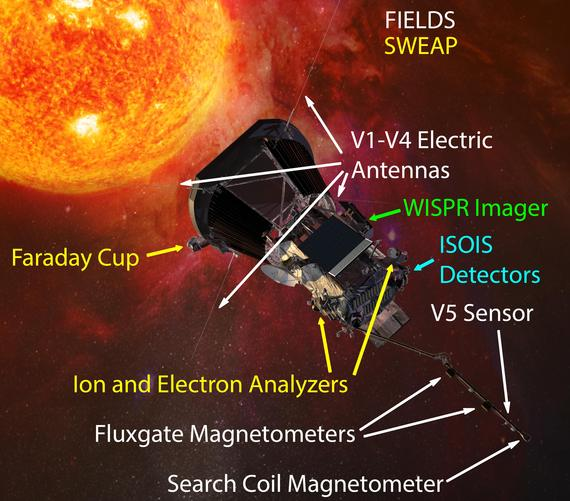
\includegraphics[width=0.9\linewidth,trim=0cm 0cm 0cm 0cm, clip=false]{./Mainmatter/Part_1/images/PSP_All_Instruments}
\cprotect\caption{Localisation des instruments de mesure sur \cacro{PSP}. Les instruments de l'expérience \cacro{FIELDS} sont notés en blanc, et ceux de \cacro{SWEAP} en jaune. Les données utilisées ici proviennent des magnétomètres à saturation (Fluxgate Magnetometers, \cacro{MAGs}) situés sur le bras et de la coupe de Faraday (Faraday Cup, \cacro{SPC}) située juste à côté du bouclier et orientée vers le Soleil. Crédits : la page web de \cacro{FIELDS} (\verb|fields.ssl.berkeley.edu|) et Johns Hopkins University Applied Physics Laboratory.}
\label{fig:sonde_PSP}
\end{figure}
 
 \cacro{FIELDS} [\cite{bale_fields_2016}] mesure le champ magnétique grâce à deux magnétomètres à saturation (\og fluxgate \fg{} en anglais), \cacro{MAGs}, mesurant la composante continue (DC) et les fluctuations à basse fréquence (MHD-ionique) du champ,  et un de type fluxmètre (\og search-coil \fg{}), \cacro{SCM}, donnant accès aux hautes fréquences (ionique-électronique). \cacro{SWEAP} [\cite{kasper_solar_2016}] est quant à elle composée d'une coupe de Faraday (\og Faraday Cup \fg{}), \cacro{SPC}, mesurant les flux globaux ionique et électronique, et d'analyseurs électrostatiques d'ions et d'électrons, \cacro{SPAN}, permettant de séparer leur état de charge. Notre étude concernant plutôt les échelles MHD, les données utilisées proviennent des instruments \cacro{MAGs} et \cacro{SPC}. 

Les données publiquement disponibles au moment où cette étude a été menée (fin 2020) provenaient des quatre premières orbites (\figref{fig:orbit_PSP}). 
\begin{figure}[!ht]
 \centering
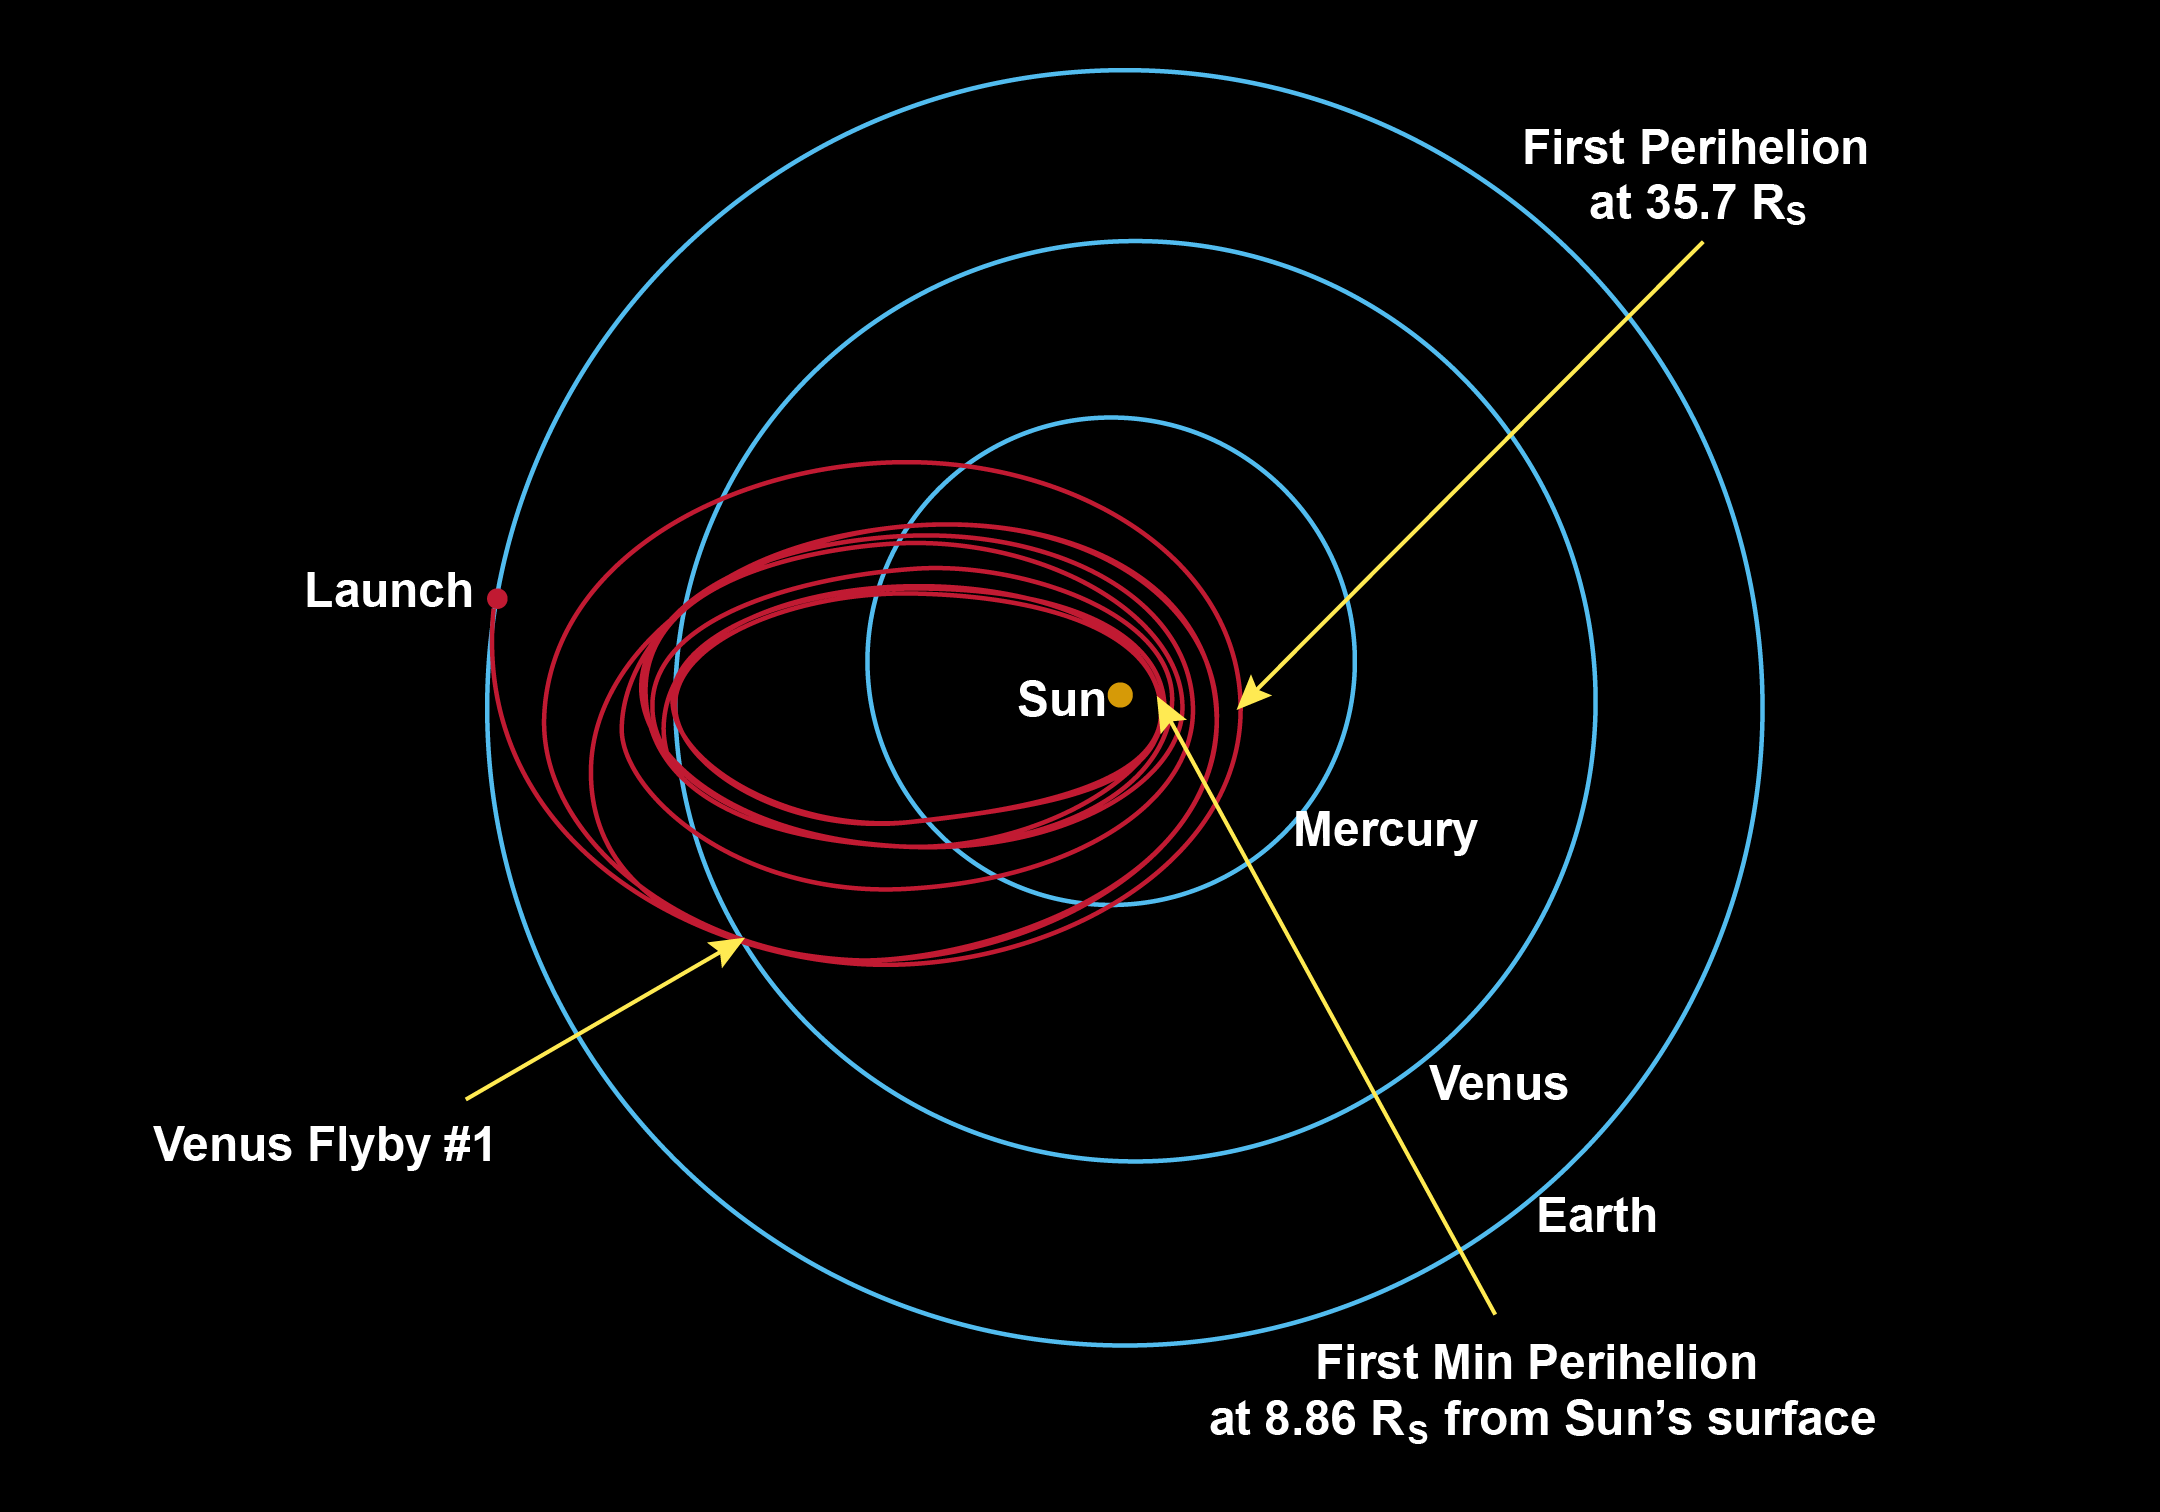
\includegraphics[width=0.9\linewidth,trim=0cm 0cm 0cm 0cm, clip=false]{./Mainmatter/Part_1/images/16-00815_MissionDesign}
\cprotect\caption{Orbites de \cacro{PSP} depuis la date de lancement, le 12 août 2018 à 7h31 \cacro{UTC}. Le premier périhélie à $\SI{35.7}{Rs}$ a été atteint le 6 novembre 2018 à 03h27 \cacro{UTC}. Crédits : la page web de \cacro{PSP} (\verb|http://parkersolarprobe.jhuapl.edu|) et Johns Hopkins University Applied Physics Laboratory.}
\label{fig:orbit_PSP}
\end{figure}
Nous avons choisi d'analyser les données relevées lorsque \cacro{PSP} était proche de son premier périhélie atteint le 6 novembre 2018 à 03h27 \cacro{UTC} vers $\SI{35.7}{Rs}$. Autour de cette position, les données sont relevées dans le vent solaire près du Soleil. Mais peu de lots de données comprenant conjointement les relevés provenant de \cacro{SPC} et ceux provenant de \cacro{MAGs} étaient assez complets pour être traités. Finalement, le jeu choisi a été relevé le 4 novembre entre 00h00 et 02h30. Les données provenant de \cacro{MAGs} y sont résolues à une cadence d'environ $\SI{7}{ms}$ sans temps manquant tandis que celles provenant de \cacro{SPC} sont résolues à $\SI{0,873}{s}$ et montrent $0.15\%$ de temps manquants situés entre 01h08 et 01h13. Ces trous seront comblés par interpolation linéaire et, afin d'avoir la même cadence, les données \cacro{MAGs} sont rééchantillonnées sur la cadence de \cacro{SPC}. Les données analysées sont montrées sur la \figref{fig:data_PSP}.  
 \begin{figure}[!ht]
 \centering
 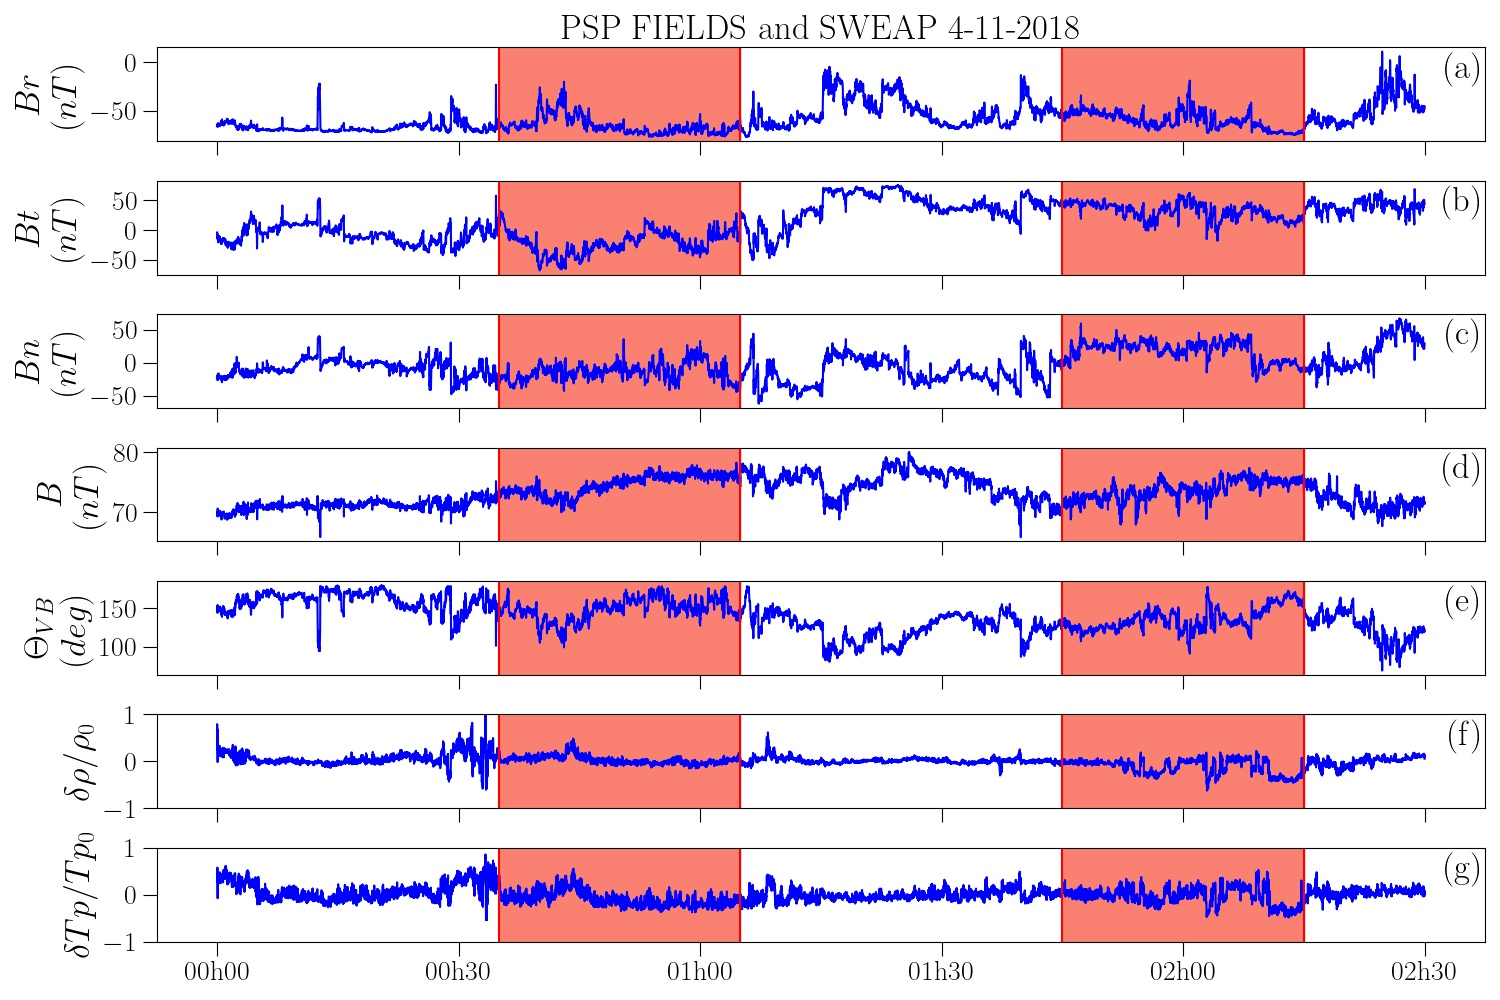
\includegraphics[width=\linewidth,trim=0cm 0cm 0cm 0cm, clip=false]{./Mainmatter/Part_1/images/Fig_04112018H_00_panel}
 \cprotect\caption{Données \cacro{PSP} mesurées dans l'héliosphère interne le 4 novembre 2018. (a) à (c) : les trois composantes du champ magnétique dans le système de représentation \cacro{RTN}. (d) : Norme du champ magnétique. (e) : angle entre le champ de vitesse du fluide et le champ magnétique. (f) et (g) : fluctuations de densité et température relative des protons. Les zones rouges représentent les sous-intervalles utilisés pour le calcul des taux de cascade.}
 \label{fig:data_PSP}
 \end{figure}

Les sous-intervalles choisis pour le calcul des taux de cascade sont marqués en rouge et sont associés à deux niveaux de compressibilité différents. La compressibilité noté $c$ est calculée en prenant l'écart-type, $\text{std}$, des fluctuations de densité, c'est-à-dire $c = \text{std}(\frac{\rho - \rho_0}{\rho_0}) = \text{std}(\frac{\delta \rho}{\rho_0})$. Le premier sous-intervalle, de 00h35 à 01h05 a une compressibilité très faible, $c \sim 8\%$, tandis que le second, de 01h45 à 02h15, est plus compressible, $c \sim 20\%$. Grâce à ces deux intervalles, nous pouvons étudier l'impact des différents niveaux de fluctuations de densité sur le taux de cascade calculé avec la loi isentrope-polytrope et la loi incompressible.

Ces choix de sous-intervalles ont été effectués en considérant un certain nombre d'hypothèses permettant de calculer un taux de cascade tout en réduisant l'incertitude du résultat. Les séries étant temporelles, on utilise l'hypothèse de Taylor\footnote{La validité de l'hypothèse de Taylor dans le vent solaire et en particulier le long de la trajectoire de \cacro{PSP} peut être remise en question [\cite{treumann_applicability_2019,chhiber_contextual_2019}] mais l'obtention d'une hypothèse de remplacement est encore une question ouverte [\cite{parashar_observations_2022}].} [\cite{taylor_spectrum_1937}] qui présuppose que les variations temporelles relevées par la sonde peuvent être interprétées comme des variations spatiales convectées par le flot de plasma à la vitesse moyenne $\boldsymbol{v_0}$. Ainsi, on peut estimer l'incrément spatial $\boldsymbol{\ell}$ à partir de l'incrément temporel $\tau $ via $ \boldsymbol{\ell} \sim \boldsymbol{v_0} \tau$. L'utilisation de l'hypothèse de Taylor donne donc accès aux échelles spatiales dans la direction moyenne du flot. Or le couplage entre le champ magnétique et le fluide implique une forte anisotropie entre les directions parallèle et perpendiculaires au champ magnétique. Par conséquent, si l'angle entre la vitesse et le champ magnétique, $\theta_{VB}$, varie trop fortement, d'importantes variations pourront apparaître dans les résultats du taux de cascade, comme l'ont observé [\cite{hadid_energy_2017}]. Les intervalles ont donc été choisis tel que $\theta_{VB}$ soit relativement stationnaire (ligne (e) de la \figref{fig:data_PSP}). On a aussi considéré des séries temporelles relativement stationnaires pour les autres quantités afin d'assurer une certaine stationnarité/homogénéité statistique. 

L'estimation des moyennes dans le calcul du taux de cascade demande une statistique suffisante, c'est-à-dire des intervalles de durée supérieure à plusieurs fois le temps de corrélation des fluctuations turbulentes [\cite{coburn_third-moment_2015}]. 
[\cite{parashar_measures_2020}] ont estimé le temps de corrélation des données relevées par \cacro{PSP} entre le 3 et le 10 novembre avec des intervalles glissants de 4h, 8h et 24h. En se fiant à cette estimation, le temps de corrélation pour les données utilisées ici (le 4 novembre entre 00h00 et 02h30) est autour de $\SI{500}{s}$, c'est-à-dire un peu moins du tiers de la longueur de nos sous-intervalles ($\SI{30}{min}$). On supposera donc que leur durée convient au calcul d'un taux de cascade. 

\begin{figure}[!ht]
 \centering
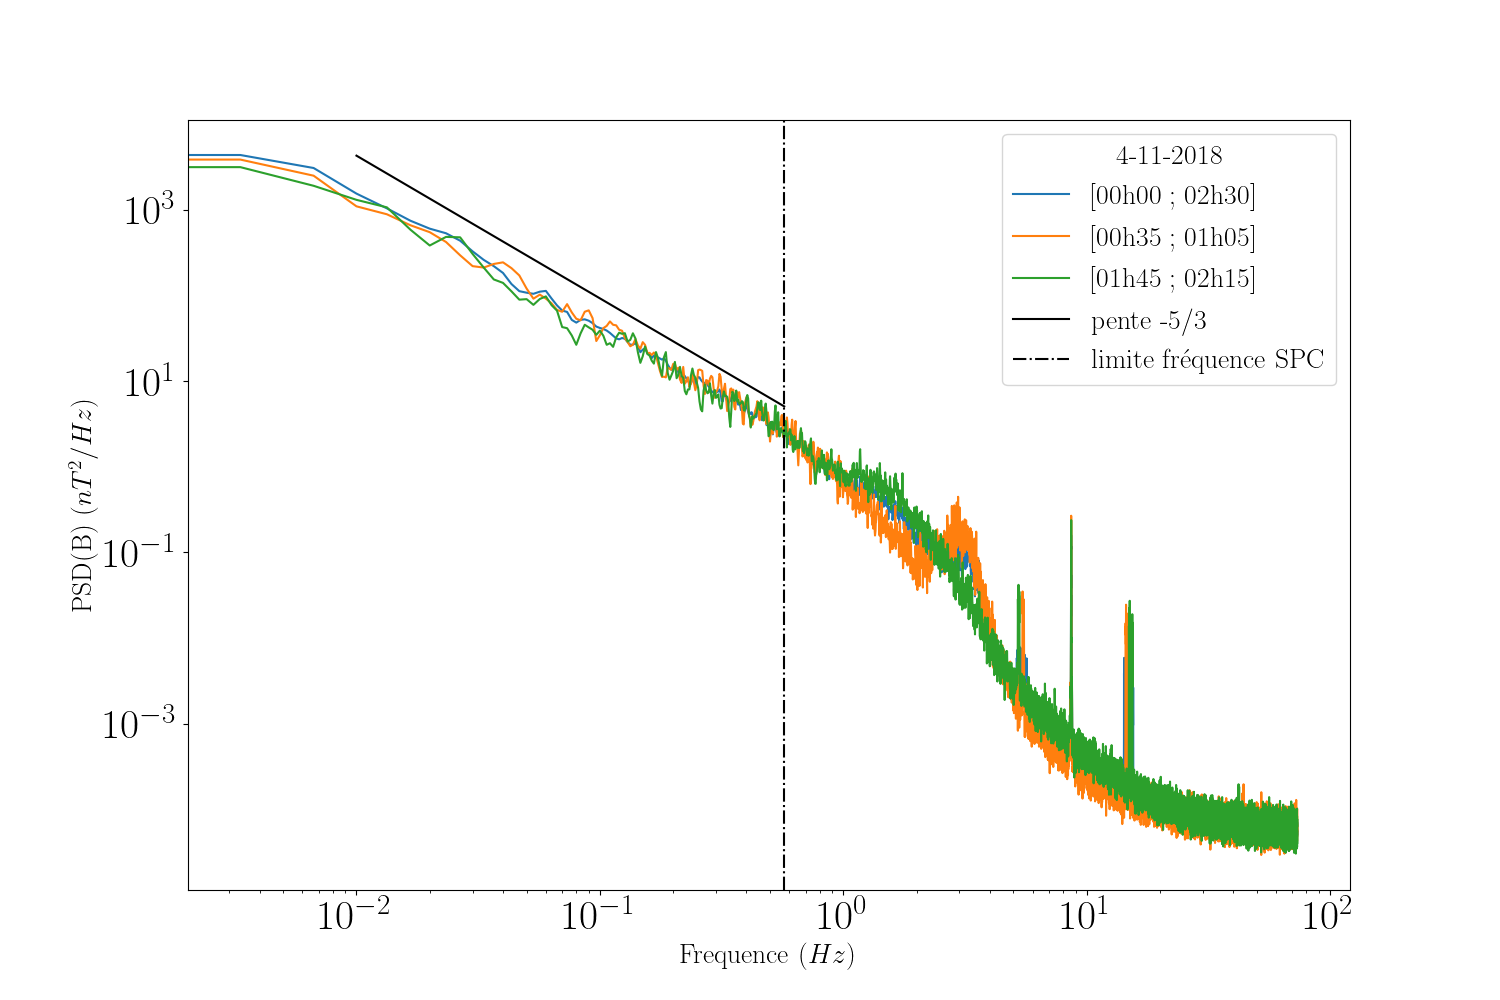
\includegraphics[width=\linewidth,trim=0cm 0cm 0cm 0cm, clip=false]{./Mainmatter/Part_1/images/Fourier2}
\cprotect\caption{Spectre des fluctuations magnétiques pour l'intervalle complet de données (bleu), et les sous-intervalles (orange et vert) obtenue avec les données \cacro{MAGs} non rééchantillonnées à la cadence de \cacro{SPC}. La ligne noire continue indique la pente attendue dans la zone MHD (spectre de type Kolmogorov en $-5/3$) et l'axe vertical la fréquence maximale accessible avec la cadence de \cacro{SPC}.}
\label{fig:spec_PSP}
\end{figure}

Sur la \figref{fig:spec_PSP}, sont tracés les spectres des fluctuations magnétiques obtenus avec les données \cacro{MAGs} non rééchantillonnées de l'intervalle complet et des deux sous-intervalles. Les fréquences qui nous intéressent sont les fréquences inférieures à la cadence de \cacro{SPC}. Pour ces fréquences, la pente des spectres est proche de $-5/3$ (attendue dans la zone \cacro{MHD}). La loi exacte du modèle \cacro{MHD} dérivée dans le Chapitre \ref{ch-13} y semble donc applicable. 
 
 \section{Comparaison des lois incompressible et compressible-isentrope-polytrope avec \ensuremath{\gamma = 1} (isotherme) et \ensuremath{\gamma = 5/3} (adiabatique)}
 \label{sec-142}

Pour ce qui est de la forme de la loi exacte, l'utilisation d'une seule sonde impose deux autres hypothèses. La première correspond à la négligence des termes sources. En effte, ces derniers ne peuvent pas être calculés à cause de leur dépendance en des dérivées locales ($\nabla$ et $\nabla'$) qui ne peuvent être estimées qu'avec des missions multi-sondes telles que \cacro{MMS} ou \cacro{CLUSTER} en orbite autour de la Terre [\cite{andres_energy_2019}]. Physiquement, une telle hypothèse pourrait avoir un impact significatif. Mais d'après l'étude numérique de [\cite{andres_energy_2019}] en turbulence MHD subsonique sur une loi exacte isentrope-isotherme formulée similairement à \eqref{eq:turb_elg_f1} (formulation qui sera considérée ici), les termes flux donnés ci-dessous \eqref{eq:obs_F1} sont dominants tandis que les autres termes sont négligeables ou se compensent. La deuxième hypothèse est celle d'isotropie des fluctuations qui permet d'intégrer tridimensionnellement la loi exacte dans une boule de rayon $\ell = |\boldsymbol{\ell}|$. Cette hypothèse simplificatrice est largement utilisée [\cite{parashar_observations_2022}] mais sa validité peut être remise en cause par l'anisotropie du plasma due au champ magnétique\footnote{Un taux de cascade incompressible intégré axisymétriquement a été investigué par \cite{andres_incompressible_2022} mais une extension compressible reste à faire.}. L'expression du taux de cascade calculée ici est alors : 
\begin{equation}
\label{eq:obs}\varepsilon = F_1 + F_2,
\end{equation}
avec
\begin{eqnarray}
\label{eq:obs_F1} F_1 &=& -\frac{3}{4|\boldsymbol{v_0}|\tau}\left<(\delta (\rho\boldsymbol{v}) \cdot \delta \boldsymbol{v}+ \delta (\rho\boldsymbol{v_A}) \cdot \delta \boldsymbol{v_A}) \delta \boldsymbol{v}  -(\delta (\rho\boldsymbol{v_A}) \cdot \delta \boldsymbol{v}  + \delta (\rho\boldsymbol{v}) \cdot \delta \boldsymbol{v_A}  ) \delta \boldsymbol{v_A} \right> \nonumber, \\ &&\\
\label{eq:obs_F2} F_2 &=& -\frac{3}{4|\boldsymbol{v_0}|\tau}\left<2 \delta \rho  \delta u  \delta \boldsymbol{v}\right>.
\end{eqnarray}
$F_1$ est la contribution dite Yaglom compressible, ne s'annulant pas dans la limite incompressible, tandis que $F_2$ est la contribution d'énergie interne, dépendant des fermetures compressibles. $\rho$ et $u$ y sont calculés pour des cas particuliers de la fermeture isentrope-polytrope définies dans la \tabref{tab:fermetures} :
\begin{itemize}
    \item incompressible (IMHD) : $\rho = \rho_0$, pas de $u$ nécessaire (cette fermeture permet de retrouver la loi \cacro{PP98}),
    \item isentrope-isotherme (CMHDi): $u = c_s^2 \ln(\frac{\rho}{\rho_0})$ obtenu avec la fermeture isentrope-polytrope et $\gamma = 1$,
    \item isentrope-adiabatique (CMHDp) : $u = \frac{c_s^2 -c_{s0}^2}{\gamma(\gamma -1)}$ obtenu avec la fermeture isentrope-polytrope et $\gamma = 5/3$.
\end{itemize}
La vitesse du son $c_s$ est obtenue grâce à la relation des gaz parfaits $c_s^2 = \gamma k_B T_p /m_p$, avec $k_B$ la constante de Boltzmann, $m_p$ la masse des protons, et $T_p$ la température locale des protons. $c_{s0}$ provient de la relation des gaz parfaits calculée avec la température moyenne des protons.
\begin{figure}[!ht]
 \centering
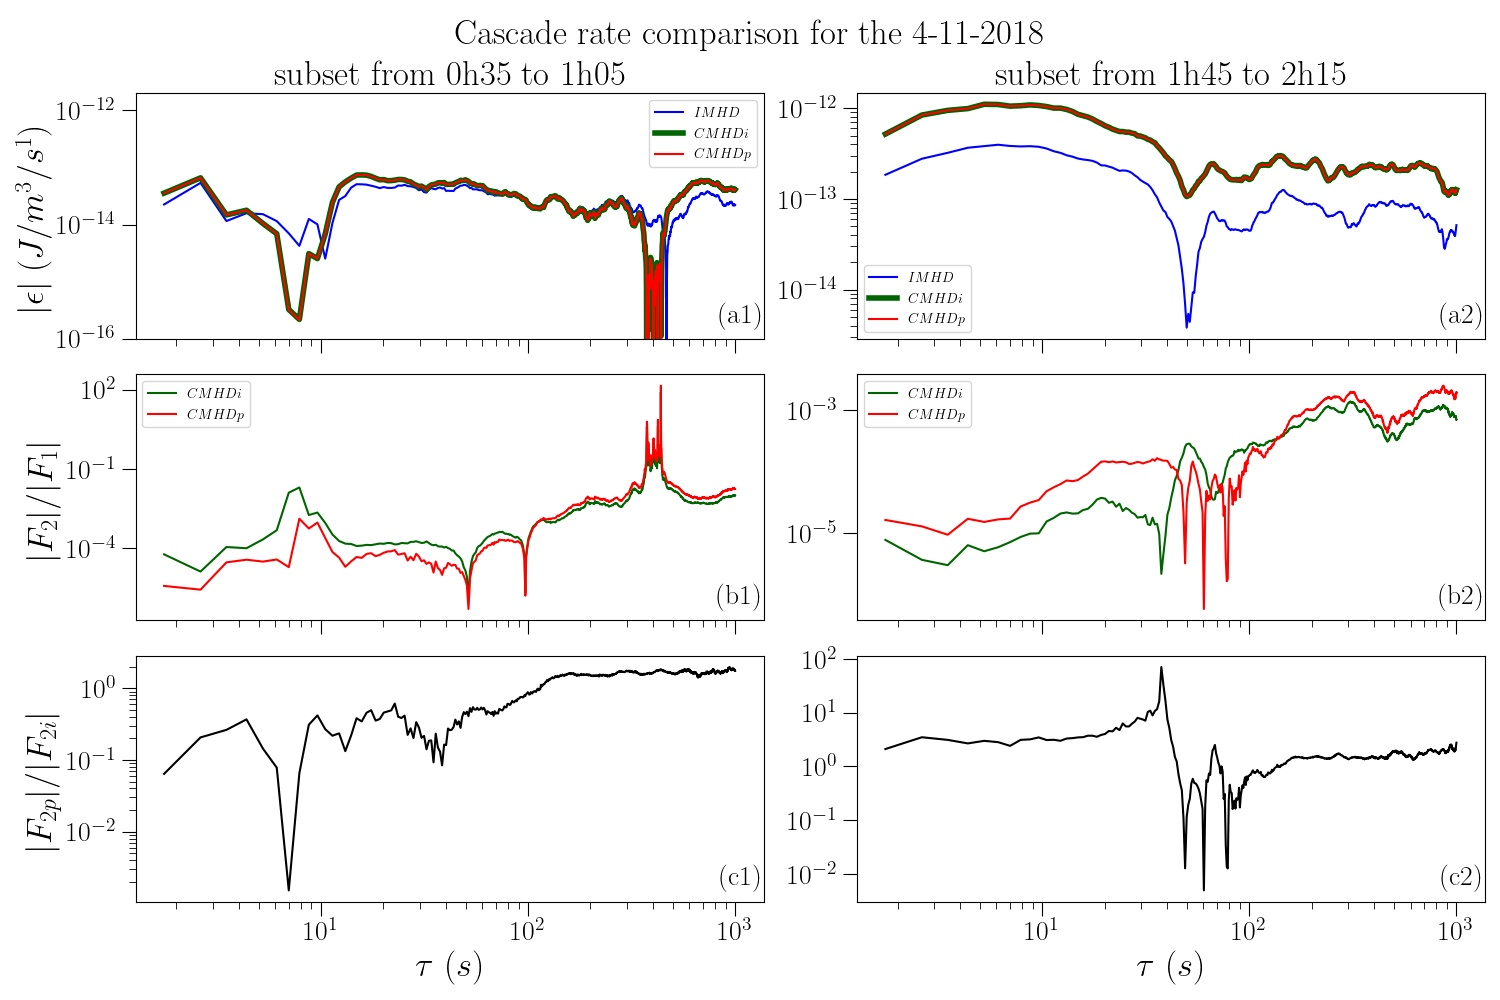
\includegraphics[width=\linewidth,trim=0cm 0cm 0cm 0cm, clip=false]{./Mainmatter/Part_1/images/Fig_04112018H_00_results}
\caption{Comparaison des taux de cascade obtenus avec l'expression de la loi exacte \eqref{eq:obs} et les différentes fermetures pour les sous-intervalles $\{$00h35–01h05$\}$ (à gauche) et $\{$01h45–02h15$\}$ (à droite). (a1)–(a2) : valeur absolue des taux de cascade obtenus avec les fermetures incompressible (IMHD) en bleu, compressibles isentrope-isotherme (CMHDi) en vert et adiabatique (CMHDp) en rouge. (b1)–(b2) : ratio entre la contribution d'énergie interne $F_2$ \eqref{eq:obs_F2} et celle Yaglom compressible $F_1$ \eqref{eq:obs_F1} dans le cas isotherme (vert) et le cas adiabatique (rouge). (c1)–(c2) : ratio entre les contributions de l'énergie interne adiabatique $F_{2p}$ et isotherme $F_{2i}$.}
\label{fig:loi_PSP}
\end{figure}

Sur la \figref{fig:loi_PSP} apparaissent les résultats pour les deux sous-intervalles, le quasi-incompressible à gauche (1) et le plus compressible à droite (2). La première ligne ((a1) et (a2)) montre l'estimation du taux de cascade avec la fermeture IMHD en bleu, la loi CMHDi en vert et CMHDp en rouge. Sur la deuxième ligne ((b1) et (b2)), la contribution d'énergie interne $F_2$ est comparée à la contribution $F_1$ dans les cas isotherme (vert) et adiabatique (rouge). L'impact de la fermeture thermodynamique n'étant portée que par $F_2$, le ratio entre les $F_2$ adiabatique ($F_{2p}$) et isotherme ($F_{2i}$) est donné sur la troisième ligne ((c1) et (c2)).

N'est représentée que la valeur absolue des différentes quantités puisque leur signe nécessite des intervalles plus longs pour statistiquement converger [\cite{coburn_third-moment_2015}, \cite{hadid_energy_2017}]. La question de l'inversion de la cascade potentiellement visualisée à travers le signe du taux ne peut donc pas être étudiée ici. Un taux $\varepsilon$ en valeur absolue quasi-constant peut par contre témoigner d'une convergence. On va donc utiliser la quasi-constance de $\varepsilon$ pour définir une zone inertielle. Pour le premier intervalle, sur le graphique (a1) de la \figref{fig:loi_PSP}, les $\varepsilon$ montrent des variations avant $\tau \sim \SI{10}{s}$ et après  $\tau \sim \SI{400}{s}$ et restent quasiment constant au centre. On supposera donc que cette zone centrale correspond à une zone inertielle. À grande échelle, ces variations proviennent de $F_1$ et se reflètent dans la brusque augmentation apparaissant sur le graphique (b1) de la \figref{fig:loi_PSP}. Ils s'avère que ces variations sont accompagnées de changements de signe. Pour le second intervalle, sur le graphique (a2) de la \figref{fig:loi_PSP}, le signe ne varie pas, il reste positif contrairement à ce que pourrait laisser présager le creux apparaissant en $\tau \sim \SI{50}{s}$. En se fiant à la quasi-constance du niveau de $\varepsilon$, nous limitons l'interprétation d'une zone inertielle à l'intervalle $\tau \in [50;800]\SI{}{s}$. 

 Le graphique (a2) de la \figref{fig:loi_PSP} met en avant le rôle de la compression dans le taux de cascade : les taux de cascade compressibles sont plus élevés d'un facteur 2 à 3 par rapport au taux incompressible, alors que le graphique (a1) de la \figref{fig:loi_PSP} provenant de données bien moins compressible montre des niveaux similaires. Cette observation coïncide avec de précédentes, issues de données du vent solaire [\cite{banerjee_scaling_2016}, \cite{hadid_energy_2017}, \cite{andres_evolution_2021}]. Par contre, les deux modèles compressibles montrent les mêmes résultats. La raison de cette convergence est révélée par les graphiques (b1) et (b2) de la \figref{fig:loi_PSP} : la contribution de $F_2$ est bien négligeable devant celle de $F_1$. Le facteur 3 observé précédemment provient donc de la prise en compte de la densité dans $F_1$.  Même si l'impact du terme dépendant de la fermeture à une importance moindre dans le taux total, nous pouvons en examiner l'effet sur les graphiques (c1) et (c2) de la \figref{fig:loi_PSP}. Aux grandes échelles ($\tau > \SI{100}{s}$), les deux fermetures apportent une contribution similaire tandis qu'à plus petite échelle (hors de la suspectée zone inertielle pour le deuxième intervalle), un ordre de grandeur de différence apparaît. Dans le cas du premier intervalle, la fermeture isotherme contribue plus que l'adiabatique tandis que dans le cas du deuxième intervalle, c'est le contraire. Une interprétation complète de cette différence de comportement ne peut être apportée avec cette étude de cas et nécessite une analyse statistique. Cette analyse, effectuée ultérieurement par \cite{brodiano_statistical_2022} dans les données \cacro{PSP} montre que $\left<F_2\right>$ (en notant $\left<\right>$ la moyenne sur les échelles et en adoptant nos notations des contributions aux taux de cascade) apparaît statistiquement un à deux ordres de grandeur en dessous de $\left<F_1\right>$, et que le facteur $\num{3}$ entre les taux compressibles et le taux incompressible n'est pas retrouvé sauf pour des cas particuliers. Les cas que nous avons étudiés semblent donc dans la norme pour le premier point vérifié, mais, pour le dernier point, notre deuxième sous-intervalle entre dans la classe des cas particuliers. Ils montrent aussi que plus la compressibilité est forte, plus $\left<F_2\right>$ peut venir concurrencer $\left<F_1\right>$ voire, pour certains cas, le surpasser. Près du Soleil, ils notent aussi que $\left<F_{2p}\right>$ est supérieur à $\left<F_{2i}\right>$ en moyenne.

Cette étude de cas préliminaire, publiée dans \cite{simon_general_2021} et validée statistiquement par \cite{brodiano_statistical_2022}, a donc permis de visualiser l'impact de la compression sur l'estimation du taux de cascade et l'apport potentiel d'une fermeture par rapport à une autre dans des données réelles du vent solaire. 

\section{Application statistique préliminaire dans des données localisées dans la magnétogaine terrestre}
\label{sec-143}

Le plasma dans la magnétogaine est plus compressible que dans le vent solaire [\cite{hadid_compressible_2018}] et d'après \cite{livadiotis_long-term_2018}, $1<\gamma<5/3$. Il est aussi exploré par de multiples missions, en particulier des missions multi-sondes comme \cacro{MMS} qui comprend quatre satellites en orbite autour de la Terre depuis 2015 (\figref{fig:MMS}). 
\begin{figure}[!ht]
 \centering
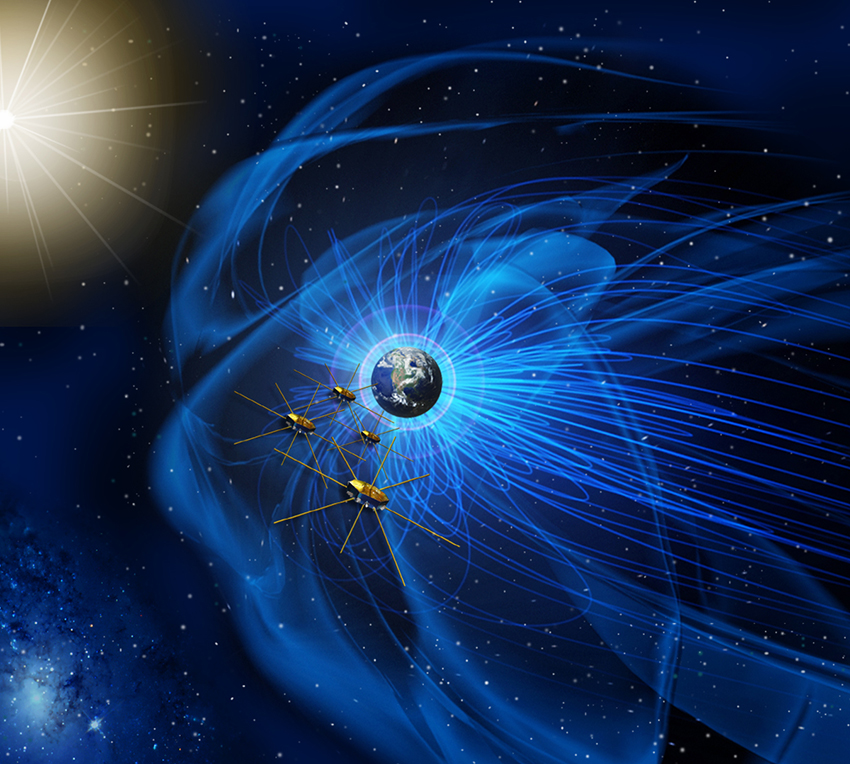
\includegraphics[width=0.7\linewidth,trim=0cm 6cm 6cm 4cm, clip=true]{./Mainmatter/Part_1/images/MMS_mission}
\cprotect\caption{Vue d'artiste de la mission \cacro{MMS}. Crédits : la page web de \cacro{MMS}/\cacro{NASA} (\verb|https://www.nasa.gov/mission_pages/mms|).}
\label{fig:MMS}
\end{figure}

À partir d'une douzaine de cas parmi ceux utilisés par \cite{andres_energy_2019}, nous avons vérifié si l'on retrouve, dans la magnétogaine, les résultats de notre étude de cas effectuée avec les données de \cacro{PSP}. Les données utilisées ont été relevées par les instruments \cacro{FPI} pour ce qui est des moments de la fonction de distribution des particules, et \cacro{FGM}, pour le champ magnétique, pendant 12 intervalles de temps entre 2015 et 2017. L'étude, similaire à celle effectuée avec les données de \cacro{PSP}, est menée séparément sur les quatre satellites de la constellation (48 résultats). 

Concernant les quantités estimées, les notations sont les mêmes que celles utilisées dans la section \ref{sec-133}. La \figref{fig:loi_MMS} montre l'emplacement des 48 résultats pour lesquels les fluctuations de densité (compressibilité $c$) varie de $20\%$ à $60\%$ (visualisé via l'échelle de couleur) dans deux diagrammes ayant pour abscisse le rapport entre les taux moyen compressible $\left<\varepsilon_{CMHDp}\right>$ obtenu avec $\gamma = 5/3$ (loi adiabatique, CMHDp) et incompressible $\left<\varepsilon_{IMHD}\right>$. Le diagramme de gauche a pour ordonnée le rapport entre les contributions d'énergie interne $\left<F_{2p}\right>$ et Yaglom compressible $\left<F_{1}\right>$ de la loi adiabatique et celui de droite le rapport entre les contributions d'énergie interne adiabatique et isentrope-isotherme, respectivement $\left< F_{2p} \right>$ et $\left< F_{2i} \right>$. 
\begin{figure}[!ht]
 \centering
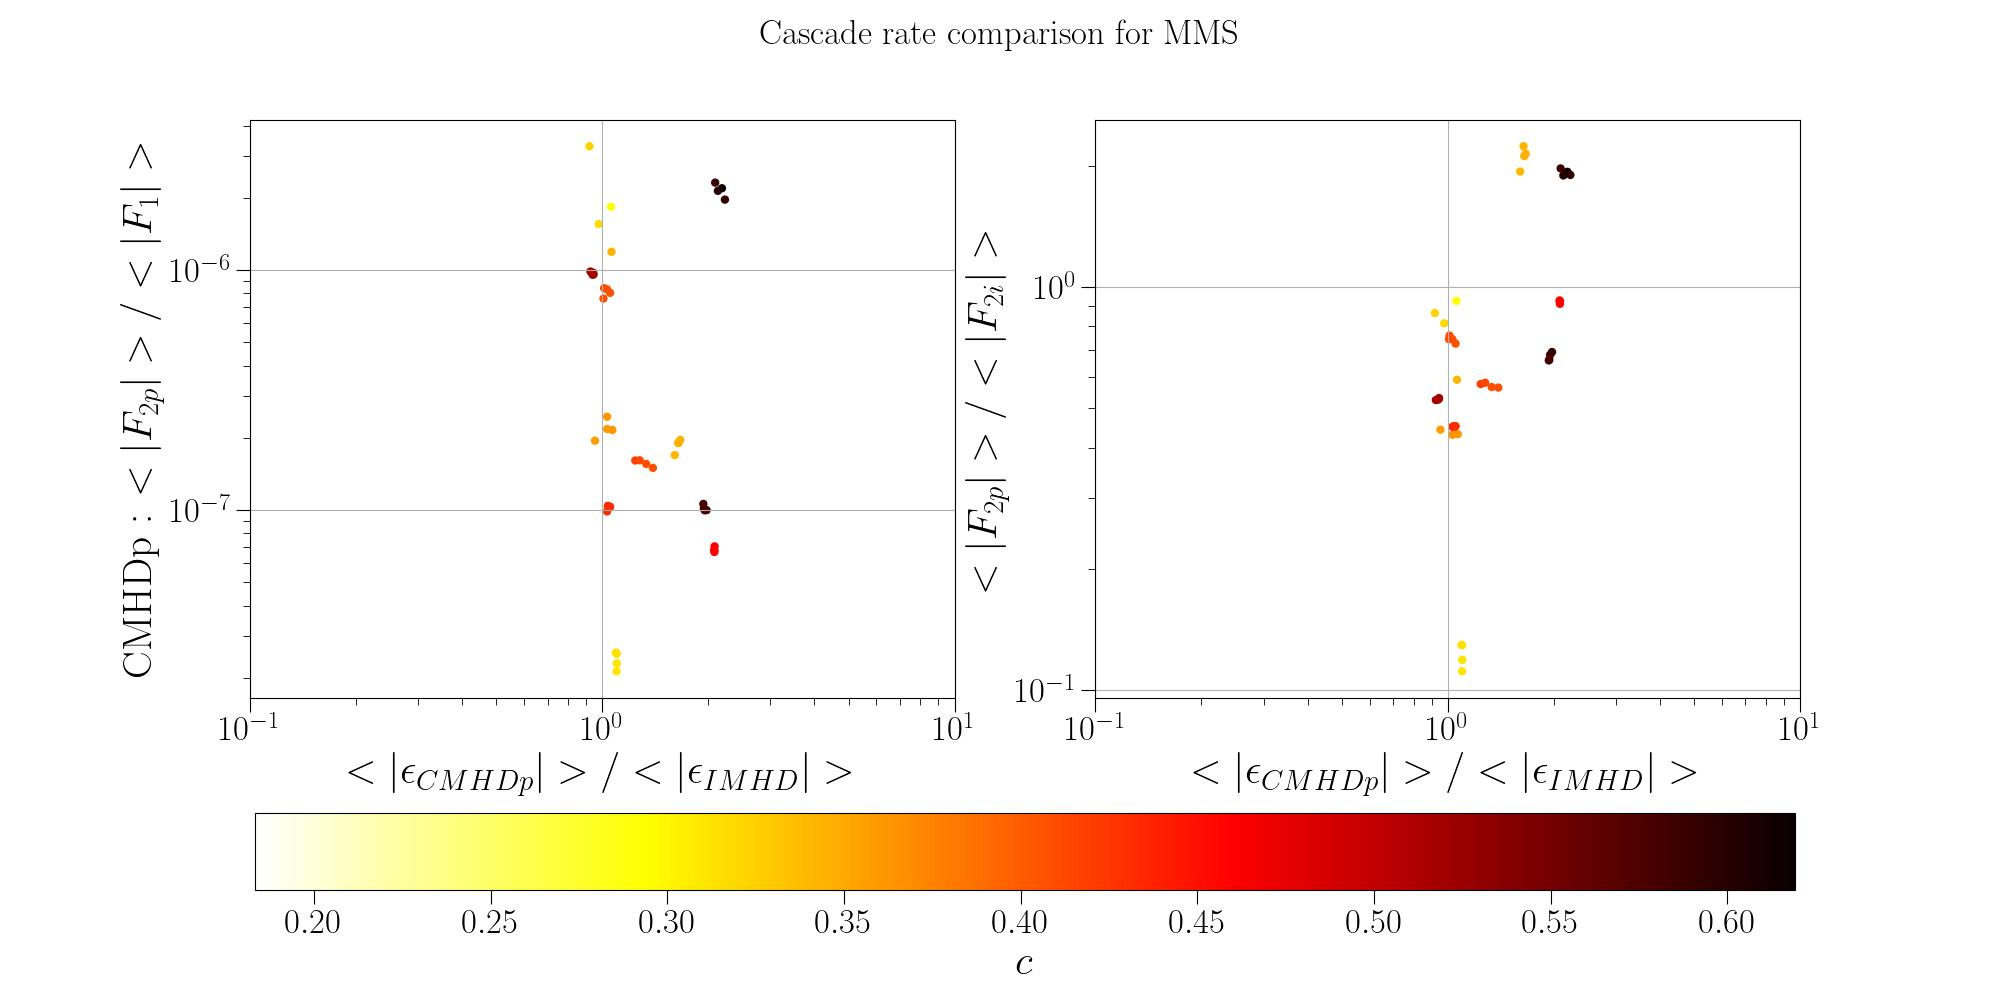
\includegraphics[width=\linewidth,trim=3cm 0cm 3cm 3cm, clip=true]{./Mainmatter/Part_1/images/cascade_comp_MMS_2}
\cprotect\caption{Résumé de l'étude statistique préliminaire menée sur 12 intervalles des quatre satellites de \cacro{MMS}. Couleurs : compressibilité $c $ de l'intervalle. Abscisses : rapport entre le taux de cascade compressible adiabatique (CMHDp, $\gamma = 5/3$) et incompressible (IMHD). À gauche : pour CMHDp, rapport entre les contributions d'énergie interne $F_2$ et Yaglom compressible $F_1$. À droite : rapport entre les contributions d'énergie interne adiabatique $F_{2p}$, et isotherme $F_{2i}$ ($\gamma = 1$).}%
\label{fig:loi_MMS}
\end{figure}

Cette étude révèle de plus importantes fluctuations de densité dans la magnétogaine que celles relevées pour les données de \cacro{PSP}. Dans les cas les plus compressibles, le taux de cascade compressible semble pouvoir doubler par rapport au taux incompressible (points rouges éloignés de la verticale centrale). Cependant, la contribution d'énergie interne moyenne y est encore plus négligeable que dans les données de \cacro{PSP}, 5 à 8 ordres de grandeurs plus faibles que la contribution Yaglom compressible moyenne comme le montre le diagramme de gauche. Sur le diagramme de droite, on voit que $\left<F_{2p}\right>$ à tendance à être un peu plus faible que $\left<F_{2i}\right>$ mais qu'il peut aussi être environ deux fois plus important. Cette dernière observation montre un comportement inverse du comportement moyen observé à tout rayon solaire dans le vent solaire par \cite{brodiano_statistical_2022}, mais demanderait plus de statistique pour être confirmée. 
 
 Cette étude dans les données de \cacro{MMS} est restée préliminaire, l'intérêt du travail ayant dévié vers l'effet de l'anisotropie de pression (voir Partie \ref{part_2}). Par la suite, une autre contribution pourrait être étudiée grâce à la constellation de satellites de \cacro{MMS} : celles des termes sources, impossible à analyser avec \cacro{PSP}. La caractéristique multi-sondes de cette mission peut en effet permettre le calcul complet des lois exactes compressibles. Cela a, par exemple, été effectué dans le cadre isotherme par \cite{andres_energy_2019}. Il serait aussi intéressant d'étudier dans les données les contributions au taux de cascade apportées par les différentes formulations ayant été analytiquement dérivées dans le chapitre précédent, en particulier les contributions des termes flux dépendant des pressions magnétique et thermodynamique, ou celle du flux de chaleur.

\newpage
\section{Synthèse de l'étude de cas observationnels issus des données de PSP}
\label{synt-14}
\fcolorbox{blue}{white}{\begin{minipage}[c]{\linewidth}
\paragraph{Données choisies : } instruments \cacro{SPC}/\cacro{SWEAP} et \cacro{MAGs}/\cacro{FIELDS} présents sur la sonde \cacro{PSP}, mesures relevées le 4 Novembre 2018, comparaison d'un intervalle quasi-incompressible et d'un plus compressible. \\

 \paragraph{Hypothèses nécessaires à l'utilisation de données in-situ issues d'une mission composée d'une seule sonde pour l'estimation de taux de cascade : } 
 \begin{itemize}
     \item taille d'intervalle supérieure à plusieurs fois le temps de corrélation des fluctuations turbulentes,
     \item hypothèse de Taylor, $\boldsymbol{\ell} \sim \boldsymbol{v_0} \tau$,
     \item angle $\theta_{VB}$ quasi-stationnaire,
     \item négligence des termes sources dans la loi exacte, valide si vent subsonique et avec la formulation f1 de la loi exacte \cacro{MHD},
     \item intégration isotrope de la loi exacte, validité à nuancer tant que l'angle $\theta_{VB}$ reste quasi-stationnaire.
 \end{itemize}
\end{minipage}}

 \fcolorbox{red}{white}{\begin{minipage}[c]{\linewidth}
 \paragraph{Loi exacte analysée : } $\varepsilon = F_1 + F_2$ avec
 \begin{eqnarray*}
  F_1 &=& -\frac{3}{4|\boldsymbol{v_0}|\tau}\left<(\delta (\rho\boldsymbol{v}) \cdot \delta \boldsymbol{v}+ \delta (\rho\boldsymbol{v_A}) \cdot \delta \boldsymbol{v_A}) \delta \boldsymbol{v}  -(\delta (\rho\boldsymbol{v_A}) \cdot \delta \boldsymbol{v}  + \delta (\rho\boldsymbol{v}) \cdot \delta \boldsymbol{v_A}  ) \delta \boldsymbol{v_A} \right> \\
  F_2 &=& -\frac{3}{4|\boldsymbol{v_0}|\tau}\left<2 \delta \rho  \delta u  \delta \boldsymbol{v}\right>
 \end{eqnarray*}
 \paragraph{Fermetures : }
 \begin{itemize}
     \item incompressible : $\rho = \rho_0$, pas de $u$ nécessaire,
     \item isentrope-isotherme : $u = c_s^2 \ln(\frac{\rho}{\rho_0})$ et $\gamma = 1$,
     \item isentrope-adiabatique : $u = \frac{c_s^2 -c_{s0}^2}{\gamma(\gamma -1)}$ et $\gamma = 5/3$.
 \end{itemize}
 
 \paragraph{Conclusion : }
 \begin{itemize}
     \item apport potentiellement substantiel de la compression via la densité dans les termes de type $F_1$ indépendant de la fermeture,
     \item apport de la fermeture important dans $F_2$ à petite échelle,
     \item $F_2$ négligeable devant $F_1$ pour les fermetures compressibles et dans les cas analysés.
 \end{itemize}
 
 Ces résultats sont publiés dans \cite{simon_general_2021}, statistiquement validés par \cite{brodiano_statistical_2022} et étendus dans la magnétogaine à travers une étude statistique préliminaire effectuée dans les données de \cacro{MMS} (section \ref{sec-133}). 
 \end{minipage}}


\chapitrestar{Conclusion}{CONCLUSION}{ch-15}
\chapter*{Conclusion}
 \addcontentsline{toc}{chapter}{Conclusion}
 \adjustmtc
\renewcommand\partie{\Partie\ CONCLUSION}
\label{ch-15}

	
%\bigskip
%\minitoc  

Depuis 1998 et la loi exacte de {\sc Politano} et {\sc Pouquet} étendant aux plasmas incompressibles, la théorie de Kolmogorov décrivant la cascade turbulente à travers des lois exactes, de multiples extensions ont été proposées prenant en compte la compressibilité. 

Dans cette partie \ref{part_1}, nous nous sommes concentrés sur l'effet de fermetures thermodynamiques dépendant d'une pression isotrope. Un premier chapitre (synthèse section \ref{synt-12}) pose le problème de la compressibilité dans les modèles fluides et analyse différentes possibilités de fermeture basées sur la théorie thermodynamique. La question qui se pose alors est celle de l'impact de la compressibilité sur la turbulence. Ma contribution pour y répondre est développée à travers les chapitres \ref{ch-13} et \ref{ch-14}. 

Dans le Chapitre \ref{ch-13} (synthèse section \ref{synt-13}), un cadre analytique est démontré à travers l'extension de la théorie des lois exactes. La stratégie mise en œuvre ne repose pas sur une fermeture thermodynamique, a contrario de celles entreprises dans la littérature [\cite{galtier_exact_2011,banerjee_exact_2013,banerjee_kolmogorov-like_2014,andres_alternative_2017}], mais plutôt, sur l'équation de densité d'énergie interne. La loi exacte résultante obtient ainsi un caractère général et la fermeture ne devient qu'un <<détail>>, une hypothèse, à ne considérer qu'à la fin du calcul en fonction du besoin. Par ce biais, est abordé l'objectif initial de cette partie du travail : obtenir une loi valable dans la zone inertielle isentrope pour une fermeture polytrope décrivant ainsi la cascade turbulente dans les plasmas de manière plus réaliste et versatile que la fermeture isotherme utilisée jusqu'à présent. La première formulation (f1) proposée pour répondre à cet objectif est inspirée du travail dans le cadre isentrope-isotherme de \cite{andres_energy_2018}. Elle a permis l'étude comparative, dans deux jeux de données issus de la mission \ac{PSP}, de l'impact de la compression et des fermetures isentropes-isotherme ($\gamma = 1$) et isentrope-adiabatique ($\gamma = 5/3$) sur la cascade turbulente. Cette étude fait l'objet du Chapitre \ref{ch-14}  (synthèse section \ref{synt-14}) où elle est étendue dans la magnétogaine à travers l'amorçage d'une étude statistique utilisant les données de MMS. L'intérêt de la formulation f1 est que les termes sources impossibles à calculer à cause des caractéristiques de la mission \ac{PSP} (une seule sonde) ont préalablement été numériquement démontrés comme négligeables dans le taux de cascade total par \cite{andres_energy_2018} dans les cadre isotherme. La deuxième formulation (f2) de la loi exacte a initialement vu le jour comme une conséquence du travail analytique qui sera présenté dans la partie \ref{part_2}, relaxant l'isotropie de pression, mais le résultat, dépendant de $p/\rho$, peut s'avérer plus adapté à l'application d'une fermeture thermodynamique. La troisième et dernière formulation (f3) est la plus récente et s'inspire du travail sur le flux de chaleur dans l'équation d'énergie interne qui s'est révélée nécessaire lors de l'étude numérique qui sera présentée dans la partie \ref{part_3}. Ce résumé des résultats obtenus avec pression isotrope reflète la structure chronologique de l'ensemble du travail effectué et présenté dans ces trois parties, la méthode scientifique mise en œuvre et les points méthodologiques utilisés. 

En termes de physique, cette partie propose un cadre d'étude de l'impact de la compression dans sa forme la plus <<simple>> : une densité variable, une pression isotrope, une énergie interne et un flux de chaleur souvent négligé. Ces grandeurs nous permettent de fermer le modèle fluide par des relations basées sur des hypothèses thermodynamiques telles que l'isentropie, l'isothermie ou la polytropie. À travers l'analyse de ces hypothèses et leur application dans les anciennes descriptions de la cascade turbulente, quatre possibilités majeures de fermeture ont émergé. La première, isentrope-isotherme est la première à avoir été utilisée dans l'extension des lois exactes [\cite{galtier_exact_2011,banerjee_exact_2013,andres_alternative_2017}]. La deuxième, isentrope-polytrope, introduite en HD [\cite{banerjee_kolmogorov-like_2014}], est celle qui nous a permis de généraliser la méthode d'obtention des lois exactes à toutes fermetures en utilisant l'équation d'énergie interne, elle prend en compte l'existence d'un $\gamma$ et reflète un peu mieux la pluralité de transformations thermodynamiques observée dans les plasmas spatiaux et astrophysiques. La troisième, polytropique, basée sur un $\gamma$ et un $\sigma$, lie le flux de chaleur au travail de pression et étend un peu plus loin les possibilités d'application des lois exactes. De la dernière, isotherme, émerge la loi exacte compressible qui semble la plus simple malgré la prise en compte des flux de chaleur. 

Pour ce qui est de l'impact de la compression et des fermetures observé dans l'étude du taux de cascade dans le vent solaire, l'étude de cas comparative montre que la compression peut jouer un rôle important dans la cascade, mais, dans les cas étudiés, la fermeture isentrope-adiabatique ou isentrope-isotherme a peu d'impact malgré le rôle qu'elle joue à travers l'énergie interne. Les termes dominants s'avèrent en effet être ceux n'en dépendant pas. On peut aussi les interpréter comme ceux subsistant dans le cas d'une fermeture isobare. Ce travail pose ainsi les bases d'une étude observationnelle, plus générale, complète et systématique, de l'impact de compression et des fermetures sur la turbulence dans les plasmas spatiaux. Cette étude est laissée au futur car le vent solaire ayant la particularité d'être peu collisionnel et magnétisé, nous nous sommes intéressés à un autre type de fermeture qui a orienté le travail dans une autre direction : celle de l'effet de l'anisotropie de pression.  












